% Options for packages loaded elsewhere
\PassOptionsToPackage{unicode}{hyperref}
\PassOptionsToPackage{hyphens}{url}
\PassOptionsToPackage{dvipsnames,svgnames,x11names}{xcolor}
%
\documentclass[
]{article}
\usepackage{amsmath,amssymb}
\usepackage{iftex}
\ifPDFTeX
  \usepackage[T1]{fontenc}
  \usepackage[utf8]{inputenc}
  \usepackage{textcomp} % provide euro and other symbols
\else % if luatex or xetex
  \usepackage{unicode-math} % this also loads fontspec
  \defaultfontfeatures{Scale=MatchLowercase}
  \defaultfontfeatures[\rmfamily]{Ligatures=TeX,Scale=1}
\fi
\usepackage{lmodern}
\ifPDFTeX\else
  % xetex/luatex font selection
\fi
% Use upquote if available, for straight quotes in verbatim environments
\IfFileExists{upquote.sty}{\usepackage{upquote}}{}
\IfFileExists{microtype.sty}{% use microtype if available
  \usepackage[]{microtype}
  \UseMicrotypeSet[protrusion]{basicmath} % disable protrusion for tt fonts
}{}
\makeatletter
\@ifundefined{KOMAClassName}{% if non-KOMA class
  \IfFileExists{parskip.sty}{%
    \usepackage{parskip}
  }{% else
    \setlength{\parindent}{0pt}
    \setlength{\parskip}{6pt plus 2pt minus 1pt}}
}{% if KOMA class
  \KOMAoptions{parskip=half}}
\makeatother
\usepackage{xcolor}
\usepackage[margin=1in]{geometry}
\usepackage{graphicx}
\makeatletter
\def\maxwidth{\ifdim\Gin@nat@width>\linewidth\linewidth\else\Gin@nat@width\fi}
\def\maxheight{\ifdim\Gin@nat@height>\textheight\textheight\else\Gin@nat@height\fi}
\makeatother
% Scale images if necessary, so that they will not overflow the page
% margins by default, and it is still possible to overwrite the defaults
% using explicit options in \includegraphics[width, height, ...]{}
\setkeys{Gin}{width=\maxwidth,height=\maxheight,keepaspectratio}
% Set default figure placement to htbp
\makeatletter
\def\fps@figure{htbp}
\makeatother
\setlength{\emergencystretch}{3em} % prevent overfull lines
\providecommand{\tightlist}{%
  \setlength{\itemsep}{0pt}\setlength{\parskip}{0pt}}
\setcounter{secnumdepth}{-\maxdimen} % remove section numbering
% definitions for citeproc citations
\NewDocumentCommand\citeproctext{}{}
\NewDocumentCommand\citeproc{mm}{%
  \begingroup\def\citeproctext{#2}\cite{#1}\endgroup}
\makeatletter
 % allow citations to break across lines
 \let\@cite@ofmt\@firstofone
 % avoid brackets around text for \cite:
 \def\@biblabel#1{}
 \def\@cite#1#2{{#1\if@tempswa , #2\fi}}
\makeatother
\newlength{\cslhangindent}
\setlength{\cslhangindent}{1.5em}
\newlength{\csllabelwidth}
\setlength{\csllabelwidth}{3em}
\newenvironment{CSLReferences}[2] % #1 hanging-indent, #2 entry-spacing
 {\begin{list}{}{%
  \setlength{\itemindent}{0pt}
  \setlength{\leftmargin}{0pt}
  \setlength{\parsep}{0pt}
  % turn on hanging indent if param 1 is 1
  \ifodd #1
   \setlength{\leftmargin}{\cslhangindent}
   \setlength{\itemindent}{-1\cslhangindent}
  \fi
  % set entry spacing
  \setlength{\itemsep}{#2\baselineskip}}}
 {\end{list}}
\usepackage{calc}
\newcommand{\CSLBlock}[1]{\hfill\break\parbox[t]{\linewidth}{\strut\ignorespaces#1\strut}}
\newcommand{\CSLLeftMargin}[1]{\parbox[t]{\csllabelwidth}{\strut#1\strut}}
\newcommand{\CSLRightInline}[1]{\parbox[t]{\linewidth - \csllabelwidth}{\strut#1\strut}}
\newcommand{\CSLIndent}[1]{\hspace{\cslhangindent}#1}
\ifLuaTeX
  \usepackage{selnolig}  % disable illegal ligatures
\fi
\usepackage{bookmark}
\IfFileExists{xurl.sty}{\usepackage{xurl}}{} % add URL line breaks if available
\urlstyle{same}
\hypersetup{
  pdftitle={Metacognitive uncertainty across the post-decisional response window},
  pdfauthor={Jesper Fischer Ehmsen1, Siebe Everaets\^{}2, Arthur S. Courtin\^{}1,3, Kelly Hoogervorst1, Francesca Fardo1*, Micah G. Allen1,4,*},
  colorlinks=true,
  linkcolor={blue},
  filecolor={Maroon},
  citecolor={Blue},
  urlcolor={Blue},
  pdfcreator={LaTeX via pandoc}}

\title{Metacognitive uncertainty across the post-decisional response
window}
\author{Jesper Fischer Ehmsen\textsuperscript{1}, Siebe Everaets\^{}2,
Arthur S. Courtin\^{}1,3, Kelly Hoogervorst\textsuperscript{1},
Francesca Fardo\textsuperscript{1*}, Micah G.
Allen\textsuperscript{1,4,*}}
\date{}

\begin{document}
\maketitle

{
\hypersetup{linkcolor=}
\setcounter{tocdepth}{3}
\tableofcontents
}
\textsuperscript{1}Center of Functionally Integrative Neuroscience
(CFIN), Department of Clinical Medicine, Aarhus University

\textsuperscript{2}KU Leuven; Faculty of Psychology and Educational
Sciences; Leuven; Belgium

\textsuperscript{3}Institute of NeuroScience, Université catholique de
Louvain, Brussels (Belgium)

\textsuperscript{4}Cambridge Psychiatry, University of Cambridge, United
Kingdom

\textsuperscript{*}Equal contributions

Corresponding author: Jesper Fischer Ehmsen
(\href{mailto:jesperfischer@outlook.dk}{\nolinkurl{jesperfischer@outlook.dk}})

\begin{center}\rule{0.5\linewidth}{0.5pt}\end{center}

This preregistration consists of three parts. The first two parts
provide justification for the experimental design and the computational
model, respectively. The third part is the main preregistration.

\begin{enumerate}
\def\labelenumi{\arabic{enumi}.}
\tightlist
\item
  \textbf{Considerations of models and empirical data from metacognitive
  perceptual decision-making tasks}
\item
  \textbf{Outline of our computational model}
\item
  \textbf{Design, methods, hypotheses, and sample size considerations of
  the current study}
\end{enumerate}

Each part is maintained in a separate document; this document includes
all three.

\begin{center}\rule{0.5\linewidth}{0.5pt}\end{center}

\section{Part 1: Perceptual Decision-Making with
Confidence}\label{part-1-perceptual-decision-making-with-confidence}

Metacognition, the ability to reflect on one's own cognitive processes,
is commonly studied through confidence ratings in decision-making tasks.
In this document we highlight empirical findings and experimental
considerations relevant to perceptual decision making with confidence
ratings.

Three main aspects characterize the relationship between confidence
ratings and choices.

\begin{enumerate}
\def\labelenumi{\arabic{enumi})}
\item
  Confidence ratings reflect a subjective probability of being correct
  or a form of self-consistency that incorporates response biases rather
  than purely objective performance
  (\citeproc{ref-CAZIOTPerceptualConfidenceJudgmentsReflectSelfconsistency2021}{Caziot
  and Mamassian 2021};
  \citeproc{ref-SANCHEZ-FUENZALIDAConfidenceReportsPerceptualDecisionMakingDissociate2025}{Sánchez-Fuenzalida
  et al. 2025};
  \citeproc{ref-MIHALIIntrospectiveInferenceCounteractsPerceptualDistortion2023a}{Mihali
  et al. 2023};
  \citeproc{ref-NAVAJASIdiosyncraticNatureConfidence2017}{Navajas et al.
  2017}).
\item
  Confidence judgments tend to underestimate relative to first-order
  accuracy (i.e., 90\% accuracy might produce 80\% confidence)
  (\citeproc{ref-SHEKHARSourcesMetacognitiveInefficiency2021}{Shekhar
  and Rahnev 2021}).
\item
  Metacognition and error-monitoring are functionally related systems,
  being confident about an error is a form of error-monitoring
  (\citeproc{ref-YEUNGMetacognitionHumanDecisionmakingConfidenceErrorMonitoring2012}{Yeung
  and Summerfield 2012};
  \citeproc{ref-FLEMINGSelfEvaluationDecisionMakingGeneralBayesianFrameworkMetacognitive2017}{Stephen
  M. Fleming and Daw 2017};
  \citeproc{ref-OZTELMetricErrorMonitoringComponentMetacognitiveProcessing2024}{Öztel
  and Balcı 2024}).
\end{enumerate}

\subsection{Models of perceptual decision making and
metacognition}\label{models-of-perceptual-decision-making-and-metacognition}

Computational models of metacognition typically fall into two
categories: \textbf{static models} based on Signal Detection Theory
(SDT) and \textbf{dynamic models} based on evidence accumulation (EA).

Static models describe choice and confidence as originating from a
static process of acquiring a fixed sample of evidence on each trial.
Confidence ratings are then assumed to be computed from this evidence
alone or in conjunction with additional independent information.

Dynamic models additionally account for response times by assuming that
evidence accumulates over time. When a decision boundary is reached
(enough evidence has been collected), a choice is made. Confidence
ratings are then thought to be generated by additional evidence
accumulation in the post-decisional time window.

Both approaches can be understood as (approximately) optimal solutions
to partially observable Markov decision processes under different
assumptions. In most perceptual decision making tasks these two types of
models are not mutually exclusive.

\subsubsection{Patterns of Confidence
ratings}\label{patterns-of-confidence-ratings}

Regardless of theoretical framework, a good metacognition model must be
able to capture several empirical patterns observed in the literature.

\begin{enumerate}
\def\labelenumi{\arabic{enumi}.}
\item
  \textbf{Performance increases with stimulus intensity}: Higher
  stimulus intensity yields higher accuracy
\item
  \textbf{Confidence curves shift in tandem with first-order choice
  curves}: As the psychometric function governing the choice
  probability, shifts from unbiased (threshold at 0) so does the
  confidence curves. The lowest confidence ratings for correct trials
  are at the stimulus value of the threshold
  (\citeproc{ref-CAZIOTPerceptualConfidenceJudgmentsReflectSelfconsistency2021}{Caziot
  and Mamassian 2021};
  \citeproc{ref-SANCHEZ-FUENZALIDAConfidenceReportsPerceptualDecisionMakingDissociate2025}{Sánchez-Fuenzalida
  et al. 2025};
  \citeproc{ref-MIHALIIntrospectiveInferenceCounteractsPerceptualDistortion2023a}{Mihali
  et al. 2023}).
\item
  \textbf{Confidence increases with stimulus intensity}: Higher stimulus
  intensities yield higher confidence ratings (conditional on accuracy,
  see below)
  (\citeproc{ref-HANGYAMathematicalFrameworkStatisticalDecisionConfidence2016}{Hangya
  et al. 2016};
  \citeproc{ref-SANDERSSignaturesStatisticalComputationHumanSenseConfidence2016}{Sanders
  et al. 2016})
\item
  \textbf{Confidence varies with accuracy}: The relationship between
  confidence and stimulus intensity depends on response correctness,
  with correct trials showing on average higher confidence than
  incorrect trials.
  (\citeproc{ref-HANGYAMathematicalFrameworkStatisticalDecisionConfidence2016}{Hangya
  et al. 2016};
  \citeproc{ref-SANDERSSignaturesStatisticalComputationHumanSenseConfidence2016}{Sanders
  et al. 2016}).

  \begin{enumerate}
  \def\labelenumii{\alph{enumii}.}
  \item
    \textbf{``Folded-X'' pattern}: Confidence sometimes increases with
    stimulus intensity for correct responses but decreases (or plateaus)
    for errors. This pattern is considered a signature of metacognition
    (\citeproc{ref-HANGYAMathematicalFrameworkStatisticalDecisionConfidence2016}{Hangya
    et al. 2016};
    \citeproc{ref-SANDERSSignaturesStatisticalComputationHumanSenseConfidence2016}{Sanders
    et al. 2016}).
  \item
    \textbf{``Double-increase'' pattern}: Confidence increases with
    stimulus intensity for both correct and incorrect responses
  \end{enumerate}
\end{enumerate}

Recent work suggest that these two patterns of confidence, could
potentially arises from different experimental manipulations
(\citeproc{ref-XUEStimulusReliabilityNotBoundaryDistanceManipulations2026}{Xue
et al. 2026};
\citeproc{ref-FUNGSimilaritiesDifferencesEffectsDifferentStimulusManipulations2025}{Fung
et al. 2025}):

\begin{itemize}
\item
  \textbf{Folded-X}: Emerges when manipulating decision-relevant
  stimulus properties (e.g., coherence in RDM).
\item
  \textbf{Double-increase}: Occurs when manipulating auxiliary
  difficulty markers (e.g., stimulus visibility).
\end{itemize}

These studies investigating patterns 4a and 4b use a confidence scale
that ranges from guessing to certain. This severely limits the
information carried by the incorrect side of the confidence curve, as we
argue in the next section. Furthermore, if participants cannot express
that they made an error, one might argue that the observed pattern does
not constitute error-monitoring, even if confidence ratings for
incorrect trials decrease as stimulus intensity increases.

Confidence patterns may reflect error-monitoring processes, but this can
only be observed when the confidence scale allows participants to
explicitly indicate that they believe they made a mistake. When
confidence is rated on a scale ranging from guessing to confident,
participants lack a clear way to report that they believe their response
was incorrect. Furthermore, confidence ratings should be administered
after the binary choice rather than simultaneously with it. Only when
the choice precedes the confidence judgment can participants first
commit to a response and then evaluate whether they may have erred. If
choice and confidence are reported simultaneously, the interpretation of
a folded X-pattern becomes ambiguous; as it could reflect participants
strategically pairing a low-confidence response with an incorrect answer
rather than detecting an error after committing to a choice.

To summarize; only a full confidence scale ranging from incorrect to
correct combined with a sequential design in which choices are followed
by confidence rating, allow subjects the ability to demonstrate
error-monitoring and thereby produce a meaningful folded-X pattern. Such
a pattern would have confidence ratings for incorrect trials fall below
the midpoint of the scale (which expresses ``guessing''). Only then
could the folded-X reflect functioning error-monitoring (confidence
decreases for errors), whereas a double-increase pattern would suggest
no error-monitoring. Below we define and describe in more detail how
experimental designs and measurement scales can influence the types of
data and the interactions one might observe.

\subsection{Confidence scales, stimulus granularity, and measurement
considerations}\label{confidence-scales-stimulus-granularity-and-measurement-considerations}

Here we outline several methodological considerations, and argue that
some of these inevitably determine the types of empirical data one can
observe.

\textbf{Confidence measurement}: Confidence is collected either
discretely or continuously. Some models of metacognition (e.g., M-ratio)
require discrete data, leading many experiments to collect or discretize
continuous confidence ratings
(\citeproc{ref-MANISCALCOSignalDetectionTheoreticApproachEstimatingMetacognitive2012}{Maniscalco
and Lau 2012};
\citeproc{ref-FLEMINGHMetadHierarchicalBayesianEstimationMetacognitiveEfficiency2017}{Stephen
M. Fleming 2017}).

\textbf{Stimulus intensity}: The main stimulus axis that determines
trial difficulty. It can be discrete or continuous.

\textbf{Confidence scale construction}: The particular anchors of a
confidence scale.

\begin{itemize}
\item
  \textbf{Half-scale confidence.} A half-scale ranges from ``guessing''
  to ``confident''. This prevents participants from expressing certainty
  about errors, they cannot indicate they are sure they made a mistake.
  Half-scales generally produce ``half-folded-X'' patterns (a flat or
  near-flat incorrect branch) rather than a full folded-X.
\item
  \textbf{Full-scale confidence.} A full scale ranges from ``confidently
  incorrect'' to ``confidently correct'', enabling participants to
  express error-monitoring. This scale can produce a full folded-X
  patterns.
\item
  \textbf{Simultaneous choice--confidence.} When choice and confidence
  are produced together, a double-increase pattern should be expected,
  because otherwise participants would have to deliberately choose the
  wrong answer.
\end{itemize}

These confidence patterns, which arise only under the aforementioned
experimental constraints, primarily reflect how incorrect trials are
distributed across stimulus intensities. Their interpretation depends
critically on the expressiveness of the confidence scale.
Error-monitoring processes can only be observed when the scale allows
participants to indicate that they believe they made a mistake. When
such responses are possible, incorrect choices can be accompanied by low
confidence (``I am confident I made a mistake'') that reflects an
awareness of being wrong. For these reasons, tasks that include many
levels of stimulus intensity together with a sufficiently expressive
confidence scale provide a parsimonious and statistically powerful
framework for investigating metacognition. In particular, the confidence
scale must allow participants to report that they believe their response
was incorrect (i.e., a full confidence scale).

\subsection{Error-monitoring}\label{error-monitoring}

Computational models of metacognition have attempted to explain
error-monitoring in different ways. A central question for these models
is why a rational agent make a mistake that they are subsequently aware
of.

Across both modeling approaches, the main answer has been to assume that
additional information is available for the confidence judgment beyond
what was used for the binary choice; if the two were identical, genuine
error-monitoring could not occur
(\citeproc{ref-FLEMINGSelfEvaluationDecisionMakingGeneralBayesianFrameworkMetacognitive2017}{Stephen
M. Fleming and Daw 2017}).

Stephen M. Fleming and Daw
(\citeproc{ref-FLEMINGSelfEvaluationDecisionMakingGeneralBayesianFrameworkMetacognitive2017}{2017})
formalized this idea in the second-order model. In this framework,
evidence for the action and evidence for the confidence rating are drawn
from a multivariate normal distribution with correlation \(\rho\)
governing the degree of information sharing. If \(\rho\) = 1, the
confidence judgment is based on the same information as the action (and
no error-monitoring is possible; i.e., a first-order model). If \(\rho\)
= 0, the confidence judgment is based on completely independent
information.

A similar idea has been proposed in the dynamic models of perceptual
decision making. In these models evidence for the initial choice arise
from a noisy accumulation process until an evidence bound is hit and a
choice is made. It is then further assumed that evidence keeps
accumulating after the choice, in a post decision evidence accumulation
window, which then gives rise to a confidence rating
(\citeproc{ref-PLESKACTwostageDynamicSignalDetectionTheoryChoice2010}{Pleskac
and Busemeyer 2010}). This theory of post-decisional evidence
accumulation (PDEA) of confidence ratings is one of the leading
theoretical accounts of the generative process underlying both choice
and confidence ratings that can explain error-monitoring
(\citeproc{ref-DESENDERUnderstandingNeuralSignalsPostdecisionalPerformanceMonitoring2021}{Desender
et al. 2021}). Below we provide a selective review of studies
investigating PDEA. Here we challenge the idea that additional
independent information is necessary for the computation of confidence
to produce the patterns of confidence described above and as a result
also error-monitoring. We end by arguing that the rater just needs
access to the action provided by the actor in order to explain the
empirical patterns.

\subsection{Post Decisional Evidence
Accumulation}\label{post-decisional-evidence-accumulation}

Several approaches have been used to determine how PDEA works. In
general, PDEA has been shown to increase metacognitive efficiency and to
have distinct electrophysiological signatures
(\citeproc{ref-DESENDERUnderstandingNeuralSignalsPostdecisionalPerformanceMonitoring2021}{Desender
et al. 2021}).

PDEA unfolds within a remarkably short temporal window. Intracranial
recordings in epilepsy patients performing mouse-tracking tasks reveal
that post-decisional confidence processing occurs within 300 - 500 ms of
choice initialization, with the pre-supplementary motor area associated
with confidence and changes of mind
(\citeproc{ref-GOUEYTESEvidenceAccumulationPresupplementaryMotorAreaInsula2025}{Goueytes
et al. 2025};
\citeproc{ref-RESULAJChangesMindDecisionmaking2009}{Resulaj et al.
2009}). Neural recordings in rhesus monkeys have further demonstrated
that anatomical regions implicated in choice formation are also the
regions associated with confidence generation
(\citeproc{ref-KIANIRepresentationConfidenceAssociatedDecisionNeuronsParietal2009}{Kiani
and Shadlen 2009}). This brief time course and overlapping neural
circuitry suggests that PDEA, rather than reflecting slow deliberative
processes, operates as a relatively automatic extension of the initial
decision dynamics.

PDEA appears to be conditional on task demands and resource constraints.
Under speed stress instructions (choice response times below 500 ms),
confidence response times are much longer, and subjects show enhanced
error monitoring, particularly for easy trials, compared to under
accuracy stress. Under accuracy stress, when subjects have sufficient
time for choice formation, choices are generally produced much slower
and confidence judgments are made after a constant time, independent of
difficulty and choice response time
(\citeproc{ref-BARANSKIProbingLocusConfidenceJudgmentsExperimentsTime1998}{Baranski
and Petrusic 1998}). Consistent with this pattern, subjects take
significantly longer to respond when they know a confidence judgment is
required compared to choice-only trials, suggesting that when not
time-pressed, evidence accumulation for choice and confidence may occur
pre-decisionally, i.e.~in a parallel or single evidence-accumulation
process
(\citeproc{ref-PETRUSICJudgingConfidenceInfluencesDecisionProcessingComparative2003}{Petrusic
and Baranski 2003};
\citeproc{ref-BARANSKITestingArchitecturesDecisionconfidenceRelation2001}{Baranski
and Petrusic 2001}).

Another way to investigate PDEA is to provide additional stiomulus
exposure after the participant has committed to a choice. Stephen M.
Fleming et al.
(\citeproc{ref-FLEMINGNeuralMediatorsChangesMindPerceptualDecisions2018a}{2018})
showed that 300 ms of additional stimulus viewing after a speed-stressed
choice (300 ms) can increase confidence efficiency (the degree to which
confidence ratings can be used to disentangle correct from incorrect
choices), with the strongest effect being a decrease in confidence
ratings for incorrect trials.

Yu et al.
(\citeproc{ref-YUDynamicsPostdecisionalProcessingConfidence2015}{2015})
found that manipulating the interval between choice and confidence
produced changes in confidence ratings, in particular decreased
confidence for errors. Additional exposure to the stimulus during this
interval did not change the quality (efficiency) of the confidence
ratings. This finding has been interpreted as internal evidence may be
sufficient for post-decisional updating and additional exposure to the
stimulus is not necessary.

In most of the highlighted studies a random dot motion stimulus is used
as the perceptual decision making task. In such tasks, participants'
performance asymptotes with exposure times of only 300--600 ms, showing
no improvement with longer presentations
(\citeproc{ref-TSETSOSActionPlanningTimescaleEvidenceAccumulation2015}{Tsetsos
et al. 2015}). Crucially, this pattern holds even when stimulus-response
mappings are manipulated, indicating that optimal decisions require only
brief stimulus exposure. However, when confidence ratings are required
participants tend to wait significantly longer before making an inital
response if not pressed for time.

Taken together, these findings suggest that when time permits, most
confidence-relevant processing may occur pre-decisionally. The most
convincing evidence for PDEA comes from conditions when participants are
time-constrained in the primary decision. In such cases, PDEA appear to
increase metacognitive efficiency primarily by decreasing confidence
ratings for incorrect choices.

\subsection{An Alternative Account: Motor Control and Choice
Variability}\label{an-alternative-account-motor-control-and-choice-variability}

While the PDEA framework offers a mechanistically parsimonious
explanation by using the same accumulation process for both choice and
confidence, we propose a more general account that does not require
additional independent information or extra PDEA. The short temporal
window of PDEA (\textasciitilde300-500 ms) coincides with timescales
consistent with motor control processes, meaning that we propose that
what is characterized as PDEA may instead reflect motor awareness. This
account can be further argued for given that under speed stress
conditions subjects produce more errors, and these errors partly arise
from reduced coordination between the central nervous system and
effectors due to the time constraints. Motor control theory,
particularly comparator models involving efference copy mechanisms,
provides a framework for understanding these errors and how agents can
become aware of them and subsequently correct them. When an agent
initiates an action, an efference copy is generated and after commitment
of the action it is compared against the expected sensory consequences,
via a forward model. Any mismatch between predicted and actual motor
output signals an error, and the magnitude of this prediction error is
an indication of the degree of confidence in the choice. Subjects can
therefore become aware that their executed action differs from their
intended choice, enabling confidence ratings below guessing, without
requiring PDEA about the stimulus itself.

From this formulation we propose that error-monitoring can arise from
choice variability, i.e.~stochasticity in the mapping from evidence to
choice. Most perceptual decision-making models assume deterministic
choices given the acquired evidence, but a stochastic choice process
allows agents to produce errors that they can subsequently be aware of.
Ordinarily, evidence variability and choice variability would be
indistinguishable from binary responses alone, however, as will be shown
below multivariate modeling of choices and confidence ratings allows
these noise sources to be distinguished.

In the following section we derive a model incorporating choice
variability, that can produce the empirical patterns of confidence and
choices described earlier. This model can be expressed as a specific
instantiation of Fleming and Daw's second-order framework
(\citeproc{ref-FLEMINGSelfEvaluationDecisionMakingGeneralBayesianFrameworkMetacognitive2017}{Stephen
M. Fleming and Daw 2017}), but without requiring independent information
while still allowing for error-monitoring.

\begin{center}\rule{0.5\linewidth}{0.5pt}\end{center}

\section{Part 2: Current Model}\label{part-2-current-model}

In this section, we first describe the general structure of ideas of
static models of perceptual decision making and confidence ratings. We
then describe, derive and simulate from our proposed model,
demonstrating that it can produce key patterns of perceptual decision
making with confidence judgements.

\subsection{Static models of
metacognition}\label{static-models-of-metacognition}

In SDT, an actor makes a binary choice on each trial \(i\),
\(a_i \in \{-1,+1\}\) based on some internal evidence \(e_i\). The
action reflects the actor's inference about the true state of the
stimulus \(D_i \in \{-1,+1\}\).

Evidence is drawn from a normal distribution, reflecting the noisy
nature of perception. The mean of this distribution reflects the true
state and scales with stimulus intensity \(X_i\). \[
e_i \sim \mathcal{N}(X_iD_i,\sigma_e)
\]

The actor then produces an action by comparing the internal evidence to
a criterion \(c\):

\[
a_i = \begin{cases}+1 & \text{if } e_i > c \\ -1 & \text{if } e_i \le c\end{cases}
\]

Within most frameworks, this criterion is thought to be static within an
experimental setting for each agent.

\paragraph{Confidence Ratings}\label{confidence-ratings}

Having made a binary choice, the agent is asked to give a confidence
judgement in that choice. A prominent approach is to assume that the
agent computes the probability that the action was correct. Stephen M.
Fleming and Daw
(\citeproc{ref-FLEMINGSelfEvaluationDecisionMakingGeneralBayesianFrameworkMetacognitive2017}{2017})
extended this framework to also account for error monitoring.

In their formulation, the confidence judgement is based on a set of
variables drawn from a multivariate normal: the evidence used for the
action \(e_i\) and a pseudo-independent information accessible only to
the rater \(r_i\). These two quantities are correlated, with \(\rho\)
governing information sharing. If \(\rho\) = 1, the confidence judgement
is based on the same information as the action; if \(\rho\) = 0, it is
based on completely independent information.

\[
\begin{bmatrix}e_i \\ r_i\end{bmatrix}\sim \mathcal{N}\left(\begin{bmatrix}X_iD_i \\ X_iD_i\end{bmatrix},\begin{bmatrix}\sigma_e^2 & \rho \cdot \sigma_e \cdot \sigma_m \\ \rho \cdot \sigma_e \cdot \sigma_m & \sigma_m^2\end{bmatrix}\right)
\]

The rater then uses this information to compute the subjective
probability of being correct, which generates a confidence rating. A
central argument for models with independent information is their
ability to explain error monitoring: agents sometimes recognize that
they have made an error and give low (even below-chance) confidence
ratings. The need for independent information follows from the fact that
a rational agent who bases both choice and confidence on the same
information (i.e., \(\rho = 1\) in the above model), and whose choices
are deterministic, cannot make an error while being aware of it. Any
information indicating that the choice is incorrect would also determine
the choice itself, thereby preventing the error.

\subsection{Efference copy (Choice Variability) model of metacognition
(EA/CV -
Meta)}\label{efference-copy-choice-variability-model-of-metacognition-eacv---meta}

\subsubsection{Choices}\label{choices}

Below we argue that independent information is not required to explain
error monitoring if we instead assume that agents show variability in
their choices given the evidence. Unlike the deterministic decision
policy usually assumed in SDT, we propose that agents have a noisy
decision process that can produce errors even when the evidence favors
the correct choice. Such errors could arise under speed stress or, more
generally, from motor noise. By introducing a stochastic choice policy
into the standard SDT framework, agents can display error monitoring
without independent information. One way to implement this is to assume
that the criterion varies from trial to trial:
\(c_i \sim \mathcal{N}(0,\sigma_c)\). This gives us:

\[
a_i = \begin{cases}+1 & \text{if } e_i > c_i \\ -1 & \text{if } e_i \le c_i\end{cases}
\]

Because both \(e_i\) and \(c_i\) are normally distributed, their
difference is also normally distributed and can be marginalized to
obtain the probability of the action:

\[
P(a = 1 \mid D_i, X_i) = \Phi\left(\frac{D_i \cdot X_i}{\sqrt{\sigma_e^2 + \sigma_c^2}}\right)
\]

Before moving on to confidence ratings, we will also assume that the
evidence distribution may be biased for each participant. This
assumption helps explain the observation that shifts in the psychometric
function of choices are accompanied by corresponding shifts in other
behavioral variables such as confidence ratings
(\citeproc{ref-CAZIOTPerceptualConfidenceJudgmentsReflectSelfconsistency2021}{Caziot
and Mamassian 2021};
\citeproc{ref-SANCHEZ-FUENZALIDAConfidenceReportsPerceptualDecisionMakingDissociate2025}{Sánchez-Fuenzalida
et al. 2025};
\citeproc{ref-MIHALIIntrospectiveInferenceCounteractsPerceptualDistortion2023a}{Mihali
et al. 2023};
\citeproc{ref-NAVAJASIdiosyncraticNatureConfidence2017}{Navajas et al.
2017}).

This leads to:

\[
e_i \sim \mathcal{N}(X_iD_i- \beta,\sigma_e)
\] And when marginalized:

\[
P(a = 1 \mid D_i, X_i) = \Phi\left(\frac{D_i \cdot X_i - \beta}{\sqrt{\sigma_e^2 + \sigma_c^2}}\right) \tag{1}
\]

From choices alone, only the sum \(\sigma_e^2 + \sigma_c^2\) can be
identified, as both noise sources equivalently flatten the psychometric
function. However, including confidence ratings allows the two to be
disentangled.

\subsubsection{Confidence ratings}\label{confidence-ratings-1}

To compute confidence ratings, we assume that the agent internally
computes the subjective probability that the choice was correct.

\[
\text{confidence} = P(\text{correct} \mid r, a) = P(D = a \mid r)
\]

Here we assume that the rater has access to a noisy readout of the
evidence: \(r_i \sim \mathcal{N}(e_i, \sigma_m)\), where \(\sigma_m\) is
metacognitive noise.

This can be shown to yield: (see the full derivation see below):

\[
P(\text{correct} \mid r_i, a, X_i) = \begin{cases}g\left(\frac{2 \cdot r_i \cdot X_i}{\sigma_e^2 + \sigma_m^2}\right) & \text{if } a = 1 \\ 1 - g\left(\frac{2 \cdot r_i \cdot X_i}{\sigma_e^2 + \sigma_m^2}\right) & \text{if } a = -1\end{cases} \tag{2}
\]

Here we assume a uniform prior on \(D\), i.e.,
\(P(D_i = 1) = P(D_i = -1) = 0.5\), representing the true state of the
world (i.e.~in the Random Dot Motion task, whether the dots are moving
up or down).

Here \(g(\cdot)\) is the inverse logit transformation, i.e.,
\(g(x)= \frac{1}{1+exp(-x)}\).

From confidence alone, only the sum \(\sigma_e^2 + \sigma_m^2\) can be
identified. However, combining choices and confidence allows estimation
of all three parameters: \(\sigma_e\), \(\sigma_c\), and \(\sigma_m\).

As can be seen from equation (2), computing the probability of being
correct requires access to the stimulus intensity \(X_i\). Although this
is assumed in some models
(\citeproc{ref-FLEMINGNeuralMediatorsChangesMindPerceptualDecisions2018a}{Stephen
M. Fleming et al. 2018}), we believe the rater does not have access to
the objective stimulus intensity. We return to this issue and present a
final formulation without this term later. Interested readers are
referred to Rausch and Zehetleitner
(\citeproc{ref-RAUSCHFoldedXpatternNotNecessarilyStatisticalSignature2019}{2019}),
where simulations are conducted with different generative processes for
the stimulus intensity.

Below we present a plate notation schematic of the proposed model,
illustrating the role of each noise parameter.

\begin{center}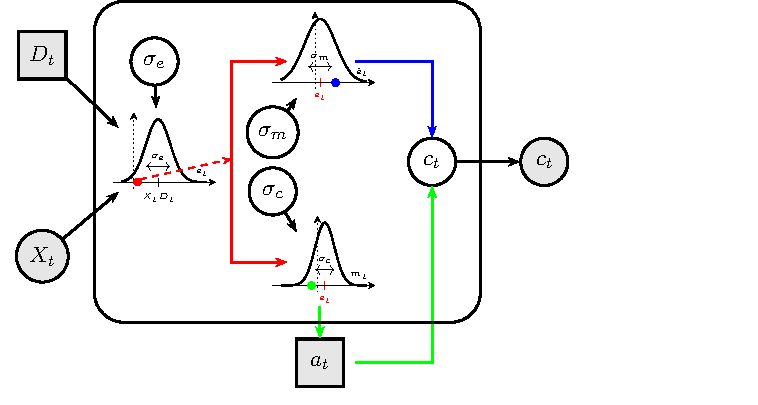
\includegraphics[width=1\linewidth]{../Figure scripts/Platenotations/platenotation} \end{center}

The model assumes that an agent is presented with a stimulus that has a
direction \(D_i\) (the true state of the world) and a strength \(X_i\).
An internal representation of the physical stimulus (evidence), \(e_i\)
(red point), is a noisy readout of the physical stimulus. This internal
evidence is then sent to the pre-motor and motor cortex, where an
efferent signal and an efference copy are produced (red split path). Due
to additional noise (\(\sigma_c\)) in the processing and transmission of
the signal to the limb, the action generated may be opposite to what the
evidence indicated (green point). Simultaneously, the efference copy may
also be subject to additional noise (\(\sigma_m\)). It is then used
together with the action to produce a prediction error in the comparator
\(C_t\), which in turn generates the confidence rating.

Next, we present simulations from the model to build intuition about the
parameters and their interact.

\subsubsection{Simulations}\label{simulations}

Below we demonstrate that the model reproduces key behavioral patterns
of choice and confidence ratings under different parameter combinations.
In brief, our simulations show that the ratio
\(\frac{\sigma_e}{\sigma_c}\) determines the degree of error monitoring
and whether the confidence patterns is a folded-X or double-increase.

\begin{itemize}
\item
  A low ratio (high \(\sigma_c\), low \(\sigma_e\)) produces folded-X
  (strong error monitoring), while a high ratio (low \(\sigma_c\), high
  \(\sigma_e\)) produces double-increase (no error monitoring).
\item
  The metacognitive noise \(\sigma_m\) flattens the confidence curves
  regardless of accuracy.
\end{itemize}

Note: For all simulations below, we assume that the bias in evidence
encoding \(\beta\) is 0. We return to this issue later, in connection
with the assumption about whether participants have access to the
objective stimulus intensity.

First, we examine the distribution of internal evidence over the
objective signed stimulus (i.e., the product of stimulus intensity and
the true state) across the two parameters governing the choices;
\(\sigma_e\) (evidence encoding ) and \(\sigma_c\) (choice variability).

\begin{center}
\includegraphics{Pre-registration_files/figure-latex/unnamed-chunk-7-1} \end{center}

From the above plot we see that \(\sigma_e\) broadens the range of
observed evidence (making it noisier for the same external stimulus);
moving down the rows, the y-axis range greatly increases. When
\(\sigma_c\) is low (left column), choices are consistent, positive
evidence is paired with positive signed stimulus (i.e.~D = 1), yielding
a correct response. As \(\sigma_c\) increases this relationship becomes
noisier, and correct and incorrect choices become less distinguishable
across the zero-evidence line and zero-signed-stimulus lines.

Another way to display this is by plotting actions instead of accuracy:

\begin{center}
\includegraphics{Pre-registration_files/figure-latex/unnamed-chunk-8-1} \end{center}

Next, we examine confidence ratings as a function of the three noise
parameters.

First, we fix \(\sigma_c = 1\) and examine how \(\sigma_e\) \&
\(\sigma_m\) change confidence ratings as a function of the signed
stimulus intensity:

\begin{center}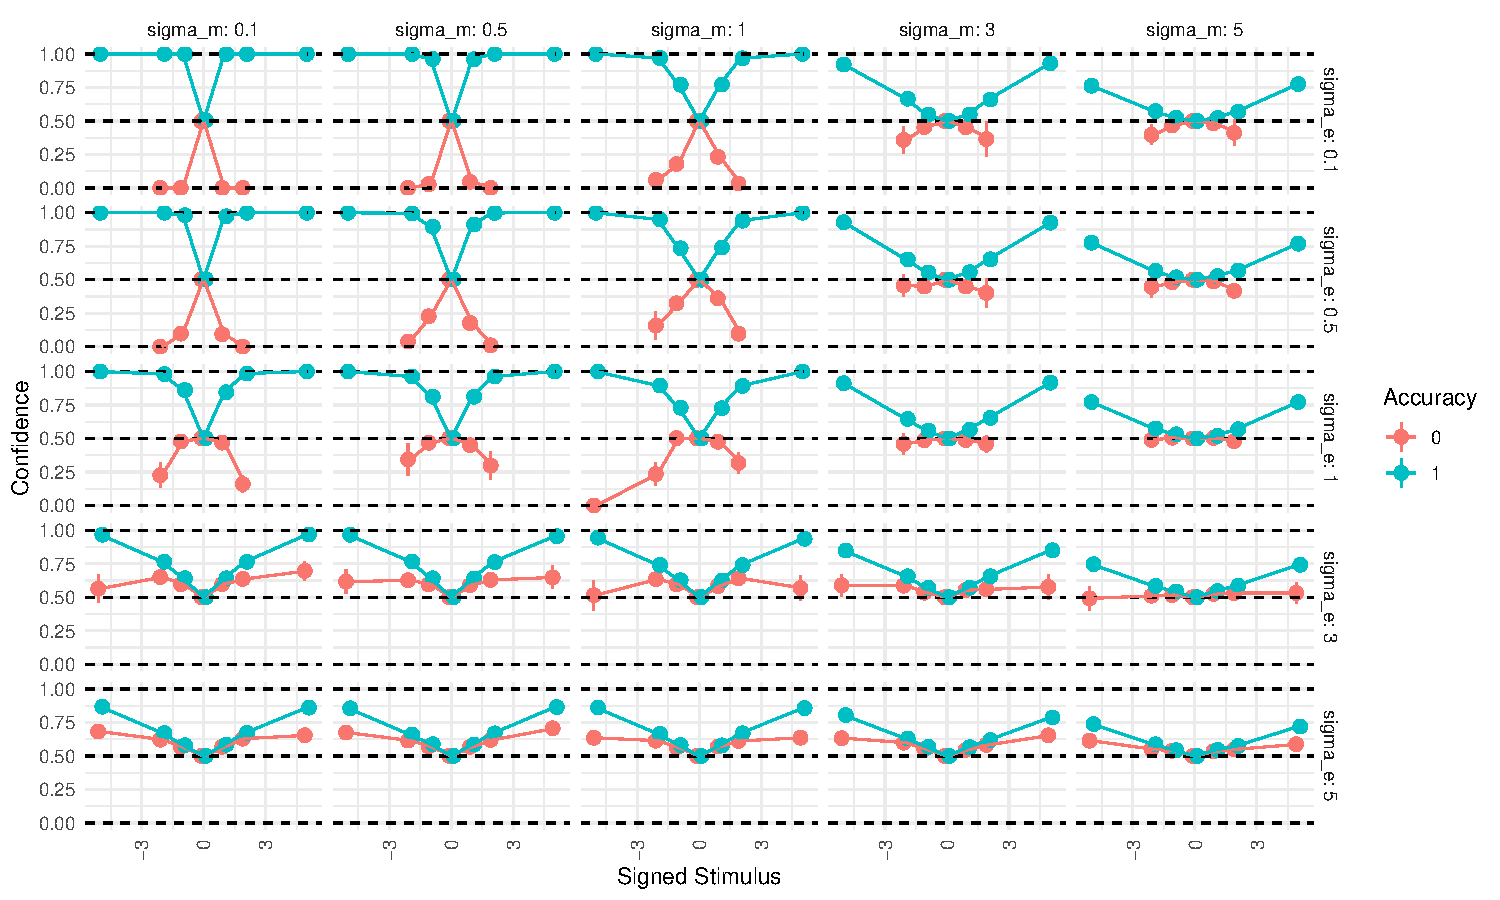
\includegraphics{Pre-registration_files/figure-latex/unnamed-chunk-10-1} \end{center}

When confidence is plotted on the signed stimulus scale, a
double-increase pattern emerges when \(\sigma_e\) is high (moving down
the facets), and a folded-X pattern appears when \(\sigma_e\) is low
(moving up the facets). As metacognitive noise (\(\sigma_m\)) increases
(moving left to right), both confidence curves become increasingly flat
(i.e., closer to 0.5) regardless of correctness.

Next, we fix \(\sigma_e = 1\) and examine \(\sigma_c\) and \(\sigma_m\):

\begin{center}
\includegraphics{Pre-registration_files/figure-latex/unnamed-chunk-11-1} \end{center}

The pattern is similar to the previous plot. A high \(\sigma_c\)
produces a folded-X, whereas lower values (especially below 1) produce a
double-increase. As before, increasing metacognitive noise
(\(\sigma_m\)) flattens both confidence curves toward 0.5 regardless of
correctness.

Lastly, we plot simulated data for varying \(\sigma_c\) and \(\sigma_e\)
with \(\sigma_m = 1\):

\begin{center}
\includegraphics{Pre-registration_files/figure-latex/unnamed-chunk-12-1} \end{center}

When \(\sigma_e = \sigma_c\) (the diagonal), it becomes difficult to
distinguish folded-X from double-increase patterns, because incorrect
trials cluster around 0.5 and show little dependence on stimulus
intensity. Correct trials increase in confidence with stimulus intensity
across all parameter combinations. In the upper triangle (where
\(\sigma_c > \sigma_e\)), folded-X patterns emerge, whereas in the lower
triangle (\(\sigma_c < \sigma_e\)), double-increase patterns emerge.

These simulations show that, in the current model, the double-increase
and folded-X patterns arise from different ratios of encoding noise to
choice variability. When choice variability is high relative to encoding
noise, a folded-X pattern arises; when choice variability is low
relative to encoding noise, a double-increase pattern arises.
Metacognitive noise (\(\sigma_m\)) is agnostic to the accuracy of the
rater and, when it increases, flattens the confidence curves regardless
of correctness.

\subsubsection{Fitting}\label{fitting}

We want to fit this model using full Bayesian inference with Stan's NUTS
sampler, treating the latent trial-by-trial evidence as parameters
estimated jointly with subject-level noise parameters. In our pilot
data, the model could be fit at the single-subject level with adequate
sampler diagnostics. However, fitting it in a hierarchical framework
(i.e., drawing subject-level parameters from group-level parameters)
produced sampling issues. Because the current project uses a sequential
sampling paradigm, a robust and efficient model is necessary. We
therefore develop a heuristic model that approximates the model
described above without requiring estimation of trial-by-trial evidence.

\subsubsection{The Heuristic model}\label{the-heuristic-model}

The computational complexity of the above model, especially in
hierarchical settings, motivates a simpler heuristic approximation. The
key challenge is that confidence requires trial-specific evidence
\(r_i\), which cannot be marginalized analytically because the random
variable is inside the inverse logit function.

The inverse logit function and the cumulative normal distribution are in
practice nearly indistinguishable up to a scaling constant, i.e.,
\(g(\cdot) \approx \Phi(\cdot / 1.7)\), as shown below:

\begin{center}
\includegraphics{Pre-registration_files/figure-latex/unnamed-chunk-13-1} \end{center}

Using this approximation, it is possible to marginalize out the
trial-by-trial evidence and arrive at a computationally less expensive
model (and a closed-form equation for the expectation of confidence)
that uses the same parameters.

With this approximation we go from equation (2) to the following:

\[
P(\text{correct} \mid r_i, a, X_i) = \begin{cases}\Phi\left(\frac{C \cdot r_i \cdot X_i}{\sigma_e^2 + \sigma_m^2}\right) & \text{if } a = 1 \\ 1 - \Phi\left(\frac{C \cdot r_i \cdot X_i}{\sigma_e^2 + \sigma_m^2}\right) & \text{if } a = -1\end{cases} \tag{3}
\]

Where \(C = \frac{2}{1.7}\).

Focusing on the case where the choice is \(a = 1\):

\[
\Phi\left(\frac{C \cdot r_i \cdot X_i}{\sigma_e^2 + \sigma_m^2}\right)
\]

We want to marginalize over \(r_i\), i.e.~calculate the expectation of
above equation, across \(r_i\). This can be done using the general
formula for the expectation of a random continuous variable.

\[
\mathbb{E(X)} = \int_{-\infty}^\infty x \ p(x) dx
\]

Substituting variables, with
\(b = \frac{CX_i}{\sigma_e^2 + \sigma_m^2}\)

\[
\int_{-\infty}^\infty \Phi(b \cdot r_i) \ p(r_i) dr_i
\]

with \(r_i \sim \mathcal{N}(\mu,\sigma)\)

This integral can be shown to have the
\href{https://www.tandfonline.com/doi/abs/10.1080/03610918008812164}{solution}:

\[
\Phi \left(\frac{\mu \cdot b}{\sqrt{1+\sigma^2 \cdot b^2}}\right)
\]

Given that
\(r_i \sim \mathcal{N}(X_iD_i - \beta, \sqrt{\sigma_m^2+\sigma_e^2})\),
we get:

\[
\Phi \left(\frac{\mathbb{E}(r_i) \cdot b}{\sqrt{1+(\sigma_e^2+\sigma_m^2) \cdot b^2}}\right)
\]

We write the expectation of \(r_i\), rather than the distributional mean
of \(r_i\) i.e., \(X_iD_i - \beta\), because this expectation will be
conditional on the choice (recall we are considering \(a_i = 1\)).

Expanding and simplifying, we obtain:

\[
\Phi\left(\frac{\mathbb{E}(r_i) \cdot CX_i}{ \sigma_e^2 + \sigma_m^2} \cdot\frac{1} {\sqrt{1 + \frac{C^2X^2_i}{\sigma_e^2+\sigma_m^2}}}\right)
\]

This equation gives the probability of being correct when the choice is
1. However, because the rater knows the actor's choice and the rater's
evidence is a noisy readout of the evidence used to generate that
choice, observing the choice provides additional information about the
underlying evidence. Mathematically, if the rater uses all available
information, the expectation of the evidence must be conditional on the
actor's choice.

Equation (3) therefore becomes:

\[
P(\text{correct} \mid a, X_i) = \begin{cases}
\Phi\left(\frac{\mathbb{E}(r_i \mid a = 1) \cdot CX_i}{\sigma_e^2 + \sigma_m^2} \cdot \frac{1}{\sqrt{1 + \frac{C^2X^2_i}{\sigma_e^2+\sigma_m^2}}}\right) & \text{if } a = 1 \\ 
1 - \Phi\left(\frac{\mathbb{E}(r_i \mid a = -1) \cdot CX_i}{\sigma_e^2 + \sigma_m^2} \cdot \frac{1}{\sqrt{1 + \frac{C^2X^2_i}{\sigma_e^2+\sigma_m^2}}}\right) & \text{if } a = -1
\end{cases} \tag{4}
\]

It can be shown that this conditional expectation equals the following
equation (for a full derivation see below):

\[
\mathbb{E}(r_i \mid a = 1) = (X_iD_i - \beta) + \rho \cdot \sqrt{\sigma_e^2 + \sigma_m^2} \cdot \lambda\left(\frac{X_iD_i - \beta}{\sqrt{\sigma_e^2 + \sigma_c^2}}\right)
\]

For \(a = -1\):

\[
\mathbb{E}(r_i \mid a = -1) = (X_iD_i - \beta) - \rho \cdot \sqrt{\sigma_e^2 + \sigma_m^2} \cdot \lambda\left(-\frac{X_iD_i - \beta}{\sqrt{\sigma_e^2 + \sigma_c^2}}\right)
\]

Here \(\lambda(x) = \frac{\phi(x)}{\Phi(x)}\), and
\(\rho = \frac{\sigma_e^2}{\sqrt{(\sigma_e^2 + \sigma_c^2)} \cdot \sqrt{(\sigma_e^2 + \sigma_m^2)}}\).

\subsubsection{Final confidence model}\label{final-confidence-model}

Substituting these conditional expectations back into equation (4) and
simplifying gives:

\[
P(correct \mid a = 1, X_i, D_i) = \Phi\left(\left[\frac{(CX_i^2D_i - C\beta X_i)}{\sigma_e^2 + \sigma_m^2} + \rho \cdot \frac{ \lambda\left(\frac{X_iD_i - \beta}{\sqrt{\sigma_e^2 + \sigma_c^2}}\right)CX_i}{\sqrt{\sigma_e^2 + \sigma_m^2} }\right] \cdot\frac{1} {\sqrt{1 + \frac{C^2X^2_i}{\sigma_e^2+\sigma_m^2}}}\right)
\]

This gives a fully marginalized model for confidence ratings (for
choices of \(a = 1\)) that depends only on the parameters
\(\Theta_1 = (\beta, \sigma_e, \sigma_c, \sigma_m)\) and the observed
data (choices \(a_i\), stimuli \(X_i\), and true states \(D_i\)),
without requiring trial-by-trial estimation of the latent evidence
variables \(e_i\) and \(r_i\).

Before interpreting this equation, we return to a key assumption
outlined just after equation (2): computing the subjective probability
of being correct requires that the participant has access to the
stimulus intensity. Below, we highlight the two \(X_i\) terms in the
equation that depend on this assumption:

\[
P(\text{correct} \mid a = 1, X_i, D_i) = \Phi\left(\frac{\left[(X_iD_i - \beta) + \rho \cdot \sqrt{\sigma_e^2 + \sigma_m^2} \cdot \lambda\left(\frac{X_iD_i - \beta}{\sqrt{\sigma_e^2 + \sigma_c^2}}\right)\right] \cdot C \mathbf{X_i}}{ \sigma_e^2 + \sigma_m^2} \cdot\frac{1} {\sqrt{1 + \frac{C^2\mathbf{X^2_i}}{\sigma_e^2+\sigma_m^2}}}\right) 
\]

These two stimulus intensity terms (shown in bold), especially the first
(which does not arise from the marginalization), ensure that at
intensity 0 the predicted confidence is always 0.5. This is a strong
assumption: it requires the agent to have access to the objective
stimulus strength, and the assumption is also inconsistent with the
empirical observation (highlighted in Part 1) that the lowest confidence
rating shifts with bias. If confidence ratings are treated as noisy,
biased subjective probabilities of being correct, the formulation above
becomes problematic because of its reliance on an objective anchor at
\(X_i = 0\). Based on these considerations, supported by empirical
validation on our pilot data below, we believe this particular stimulus
intensity term, which rests on an unjustified assumption, needs to be
addressed.

One possible solution is to assume that the agent has a noisy readout of
stimulus strength, \(\hat{X} \sim p(\hat{x}|\theta,c)\). The difficulty
with this formulation is defining the probability distribution of the
internal stimulus intensity. This distribution must be positively
bounded (\(\hat{X} > 0\)), which introduces an arbitrary distributional
choice and, more importantly, makes it nontrivial to marginalize the
trial-by-trial readout. An alternative approach would be to replace the
stimulus intensity with a participant-specific constant, serving as a
placeholder for idiosyncratic differences in how participants use
stimulus intensity information beyond what they should have access to.

Instead, we assume that agents do not have access to this stimulus
intensity and fix it to 1. This approach circumvents the computational
difficulties mentioned above while remaining consistent with what the
agent is assumed to have access to. It also allows the model to
accommodate the empirical observation that the confidence curve follows
the psychometric function of the binary choices. Below, we show that in
our pilot data, the two models (fixing this stimulus intensity to 1
versus letting it vary with the true stimulus intensity) have equivalent
approximate leave-one-out cross-validation performance.

The final equations becomes:

\[
P(\text{correct} \mid a = 1, X_i, D_i) = \Phi\left(\left[\frac{(CX_iD_i - C\beta)}{\sigma_e^2 + \sigma_m^2} + \rho \cdot \frac{ \lambda\left(\frac{X_iD_i - \beta}{\sqrt{\sigma_e^2 + \sigma_c^2}}\right)C}{\sqrt{\sigma_e^2 + \sigma_m^2} }\right] \cdot\frac{1} {\sqrt{1 + \frac{C^2}{\sigma_e^2+\sigma_m^2}}}\right) \tag{7a}
\]

which for \(a = -1\) becomes:

\[
P(\text{correct} \mid a = -1, X_i, D_i) = 1-\Phi\left(\left[\frac{(CX_iD_i - C\beta)}{\sigma_e^2 + \sigma_m^2} - \rho \cdot \frac{ \lambda\left(-\frac{X_iD_i - \beta}{\sqrt{\sigma_e^2 + \sigma_c^2}}\right)C}{\sqrt{\sigma_e^2 + \sigma_m^2} }\right] \cdot\frac{1} {\sqrt{1 + \frac{C^2}{\sigma_e^2+\sigma_m^2}}}\right) \tag{7b}
\]

with:

\[
\lambda(x) = \frac{\phi(x)}{\Phi(x)} \\
C = \frac{2}{1.7}
\]

In the above formula it is noteworthy that the terms inside the
cumulative normal distribution function have clear interpretations.

First, the common factor is a correction for marginalization:

\[
K_i = \frac{1}{\sqrt{1 + \frac{C^2}{\sigma_e^2+\sigma_m^2}}}
\]

The two remaining terms have direct cognitive interpretations. Returning
to equation (3) (now with \(X_i = 1\)), the first term from equations
(7a/7b) is the expectation of the log-likelihood ratio (the argument
inside \(\Phi(\cdot)\)). It can be interpreted as the \textbf{prior
belief about being correct based purely on the stimulus}, before any
information about the action is taken into account:

\[
I_i = \mathbb{E}\left(\frac{C \cdot r_i}{\sigma_e^2 + \sigma_m^2}\right) = \frac{C(X_iD_i - \beta)}{\sigma_e^2 + \sigma_m^2}
\]

The second term updates this prior using the information carried by the
action via the efference copy:

\[
S_i = \pm\rho \cdot \frac{\lambda\left(\pm\frac{X_iD_i - \beta}{\sqrt{\sigma_e^2 + \sigma_c^2}}\right)C}{\sqrt{\sigma_e^2 + \sigma_m^2}}
\]

This term functions as an \textbf{internal action prediction error}: it
reflects the discrepancy between the action the evidence predicted and
the action actually executed, as observed through the noisy efference
copy channel. Its magnitude is governed by the inverse Mills ratio
\(\lambda(\cdot)\), which is large when the action was surprising given
the evidence (i.e., errors at high stimulus intensity) and near zero
when the action was expected (i.e., correct responses at high stimulus
intensity). Confidence in probit space is therefore the sum of a prior
and a prediction error, scaled by the correction factor:

\[
\Phi^{-1}(\mu_{c_i}) = (I_i + S_i) \cdot K_i
\]

This is analogous to a reinforcement learning rule where a prior value
estimate is corrected by a prediction error, but here no external
feedback is necessary; the efference copy itself serves as the internal
reference signal. The addition of action information to the confidence
computation was proposed in the second-order rater model of Stephen M.
Fleming and Daw
(\citeproc{ref-FLEMINGSelfEvaluationDecisionMakingGeneralBayesianFrameworkMetacognitive2017}{2017}),
with empirical support from reanalysis of behavioral data. The present
formulation makes the mechanism explicit: the efference copy supplies
the prediction error.

For completeness, we show the magnitude of these two terms as a function
of signed stimulus intensity. For a range of stimulus intensities
\(U(0.05,1)\), we show how both \(I_i\) and \(S_i\) vary with choice
correctness.

\begin{center}
\includegraphics{Pre-registration_files/figure-latex/unnamed-chunk-15-1} \end{center}

Here \(\sigma_m\) and \(\sigma_e\) have qualitatively the same effect on
\(I_i\), both reduce the strength of the relationship between signed
stimulus intensity and average evidence in favor of the true state.

Next, we examine how the parameters influence the second term \(S_i\).
First, we plot varying levels of \(\sigma_m\) with \(\sigma_e = 0.5\)
and \(\sigma_c = 0.5\)

\begin{center}
\includegraphics{Pre-registration_files/figure-latex/unnamed-chunk-16-1} \end{center}

In the above plot, each quadrant corresponds to a different state of the
decision process. Green quadrants indicate correct responses; red
quadrants indicate errors. Line color represents different levels of
metacognitive noise \(\sigma_m\). The magnitude of \(S_i\) is uniformly
attenuated as \(\sigma_m\) increases.

\begin{center}
\includegraphics{Pre-registration_files/figure-latex/unnamed-chunk-17-1} \end{center}

The same quadrant structure applies. The plot shows that increasing
either \(\sigma_e\) or \(\sigma_c\) reduces the magnitude of \(S_i\).

To summarize, confidence in this model is the sum of a stimulus-based
prior \(I_i\) and an action-based prediction error \(S_i\), scaled by
the marginalization factor \(K_i\). The prediction error is largest for
incorrect responses at high stimulus intensity and smallest for correct
responses at high stimulus intensity. This pattern has implications for
how physiological responses, particularly pupil dilation, may track the
decision process.

\paragraph{Additional parameters}\label{additional-parameters}

We introduce 5 additional parameters.
\(\Theta_2 = (\kappa_c, \gamma, \mu_{\beta}, c_0,c_1)\).

\begin{itemize}
\item
  \(\gamma\) is the lapse rate on the binary choices, a stimulus
  independent factor that shifts the asymptote of the psychometric
  function away from certainty i.e., the asymptotes become \(\gamma\)
  and \(1-\gamma\).
\item
  \(\mu_{\beta}\) is a metacognitive bias parameter, serving as an
  independent vertical shift of confidence ratings.
\item
  \(\kappa_c\) is the precision of the ordered beta likelihood.
\item
  \(c_0\),\(c_1\) are the two cutpoints for the ordered beta likelihood.
  These two parameters help generalize the beta-distribution to outcomes
  that include 0 and 1 ratings.
\end{itemize}

See
(\citeproc{ref-KUBINECOrderedBetaRegressionParsimoniousWellFittingModel2023}{Kubinec
2023}) for the ordered beta likelihood.

The complete set of parameters for the model is:

\[
\begin{aligned}
\Theta_s = \begin{bmatrix}
           \beta_s \\
           \sigma_{e_s} \\
           \sigma_{c_s} \\
           \sigma_{m_s} \\
           \mu_{\beta_s} \\
           \kappa_{c_s} \\
           \gamma_s 
         \end{bmatrix} 
         &\sim 
         \mathcal{N}(\mu_{\Theta},\Sigma_{\Theta}) \\
\text{where } \quad & \beta_s  \in [-1,1], \sigma_{e_s} >0, \sigma_{c_s} >0, \sigma_{m_s} > 0, \\
& \mu_{\beta_s} \in \mathbb{R}, \kappa_{c_s} > 0, \gamma_s \in [0,0.5] \\
& (c_{1_s} , c_{0_s}) \sim \delta([1,10,1])
\end{aligned}
\]

In this formulation, \(\mathcal{N}\) denotes a multivariate normal
distribution with mean and covariance. All parameter constraints are
enforced through transformations: positively constrained parameters are
exponentiated, and bounded parameters are transformed with the inverse
logit function and scaled appropriately. The cutpoint constraints are
imposed via a Dirichlet prior (\(\delta()\)). Note that cutpoints are
sampled on a subject-by-subject basis.

The priors of the model are as follows:

\[
\begin{aligned}
\mu_{\beta} &\sim \mathcal{N}(0, 0.5) & \text{(group mean of threshold)} \\
\mu_{\sigma_{e_s}} &\sim \mathcal{N}(-2, 2) & \text{(group mean of encoding uncertainty)} \\
\mu_{\sigma_{c_s}} &\sim \mathcal{N}(-2, 2) & \text{(group mean of choice variability)} \\
\mu_{\sigma_{m_s}} &\sim \mathcal{N}(-2, 2) & \text{(group mean of meta uncertainty)} \\
\mu_{\beta_c} &\sim \mathcal{N}(0, 0.5) & \text{(group mean of meta bias)} \\
\mu_{\gamma_s} &\sim \mathcal{N}(2, 2) & \text{(group mean of lapse rate)} \\
\mu_{\kappa_c} &\sim \mathcal{N}(-4, 2) & \text{(group mean of confidence precision)} \\
\end{aligned}
\]

\[
\begin{aligned}
\tau_{\beta} &\sim \mathcal{N}(1, 1) & \text{(Between subject SD of threshold)} \\
\tau_{\sigma_{e_s}} &\sim \mathcal{N}(1, 1) & \text{(Between subject SD of encoding uncertainty)} \\
\tau_{\sigma_{c_s}} &\sim \mathcal{N}(1, 1) & \text{(Between subject SD of choice variability)} \\
\tau_{\sigma_{m_s}} &\sim \mathcal{N}(1, 1) & \text{(Between subject SD of meta uncertainty)} \\
\tau_{\beta_c} &\sim \mathcal{N}(1, 1) & \text{(Between subject SD of meta bias)} \\
\tau_{\gamma_s} &\sim \mathcal{N}(1, 1) & \text{(Between subject SD of lapse rate)} \\
\tau_{\kappa_c} &\sim \mathcal{N}(1, 1) & \text{(Between subject SD of confidence precision)} \\
\end{aligned}
\]

\begin{itemize}
\tightlist
\item
  \(\mathbf{R} \sim \mathrm{LKJ}(\eta = 2)\) (correlation matrix for the
  multivariate normal distribution.)
\item
  \(z_{expo} \sim \mathcal{N}(0, 1)\) (participant deviations)
\item
  \(c_0, c_{1}\): see Dirichlet prior in Stan code
\end{itemize}

The full model is

\[
\begin{aligned}
P(a = 1) &= \Phi\left(\frac{D_i \cdot X_i- \beta_s}{\sqrt{\sigma_{e_s}^2 + \sigma_{c_s}^2}}\right) \\
\mu_{c_i} &= \begin{cases}\Phi\left((I_i-S_i)\cdot K_i\right) & \text{if } a_i = 1 \\ 
1 - \Phi\left((I_i+S_i)\cdot K_i\right) & \text{if } a_i = -1\end{cases} \\
a_i &\sim \mathcal{bernoulli}(p(a_i = 1)) \\
Conf_i &\sim \mathcal{ord\beta}(\mu_{c_i},\kappa_{c_s},c_{0_s},c_{1_s})
\end{aligned}
\]

with

\[
I_i = \frac{(CX_iD_i - C\beta)}{\sigma_{e_s}^2 + \sigma_{m_s}^2}, \quad
S_i = -\rho_s \cdot \frac{ \lambda\left(-\frac{X_iD_i - \beta_s}{\sqrt{\sigma_{e_s}^2 + \sigma_{c_s}^2}}\right)C}{\sqrt{\sigma_{e_s}^2 + \sigma_{m_s}^2} }, \quad
K_i = \frac{1} {\sqrt{1 + \frac{C^2}{\sigma_{e_s}^2+\sigma_{m_s}^2}}}
\]

Next, we verify the marginalized heuristic model by simulating data from
equation (2) (with \(X_i = 1\)), averaging across the signed stimulus
axis, and displaying the predictions of the marginalized heuristic model
for the same parameter values (\(\Theta_1\)).

In the first validation step, we simulate from different combinations of
noise parameters (shown as facets).

\begin{center}
\includegraphics{Pre-registration_files/figure-latex/unnamed-chunk-18-1} \end{center}

The above plot shows results from averaging \ensuremath{5\times 10^{5}}
simulated trials from equation (2) for each bin of the signed stimulus
intensity scale (dots are means with approximate 95\% intervals). The
thick solid lines represent the marginalized heuristic model
predictions.

Next, we simulate using fixed noise parameters and vary the bias
\(\beta\). Note that here we display the action rather than the accuracy
of the choice.

\begin{center}
\includegraphics{Pre-registration_files/figure-latex/unnamed-chunk-19-1} \end{center}

The above plot shows results from averaging \ensuremath{5\times 10^{5}}
simulated trials from equation (2) for each bin of the signed stimulus
intensity scale (dots are means with approximate 95\% intervals). The
thick solid lines represent the marginalized heuristic model
predictions.

\subsubsection{Model for the current
experiment.}\label{model-for-the-current-experiment.}

In the current experiment, participants are presented with a random dot
kinematogram on each trial and asked to choose which direction the
majority of dots are moving. After an experimental delay
(post-decisional response window), participants give a confidence
rating. We aim to test whether this post-decisional response window
changes the metacognitive noise and metacognitive bias parameters of the
above model. This is implemented as follows:

\[
\sigma_{m_t}  = \sigma_{m_s} + \Delta{\sigma_{m_s}} \cdot PDW_t\\
\mu_{\beta_t} = \mu_{\beta_s} + \Delta{\mu_{\beta_s}} \cdot PDW_t
\]

The subject-level changes due to the post-decisional window (PDW) are
drawn from additional group-level parameters in the multivariate normal
distribution described above. These group-level parameters are given the
following priors:

\[
\begin{aligned}
\mu_{\Delta{\sigma_{m_s}}} &\sim \mathcal{N}(0, 0.5) & \text{(group mean of effect of PDW on meta uncertainty)} \\
\mu_{\Delta{\mu_{\beta_c}}} &\sim \mathcal{N}(0, 0.5)  & \text{(group mean of effect of PDW on meta bias)} \\
\tau_{\Delta{\sigma_{m_s}}} &\sim \mathcal{N}(0, 0.5) & \text{(Between subject SD of effect of PDW on meta uncertainty)} \\
\tau_{\Delta{\mu_{\beta_c}}} &\sim \mathcal{N}(0, 0.5)  & \text{(Between subject SD of effect of PDW on meta bias)} \\
\end{aligned}
\]

\begin{itemize}
\item
  PDW denotes the post-decisional response window.
\item
  \({\Delta{\sigma_{m_s}}}\) and \(\Delta{\mu_{\beta_c}}\) denote the
  change in metacognitive noise and metacognitive bias due to PDW,
  respectively.
\end{itemize}

Next, we investigate how this model, with metacognitive noise and
metacognitive bias varying by PDW, fits our pilot data. The first step
is model comparison using approximate leave-one-out cross-validation
between the model assuming the rater has access to the objective
stimulus intensity and the reduced model where \(X_i = 1\).

\subsubsection{Model comparison}\label{model-comparison}

As a sanity check on the \(X_i = 1\) assumption, we fitted both
hierarchical models to our pilot data and computed approximate
leave-one-out cross-validation. The two models were virtually
indistinguishable, with the difference in expected log predictive
density being -1.58 \(\pm\) 9.9. A difference below \(-4\) or more than
two standard errors from zero is generally considered evidence for one
model over the other (REF); thus, at least in our pilot data, there is
no difference in predictive performance. To further examine the
distinction, we plot all pairwise parameter estimates below together
with the identity line.

\begin{center}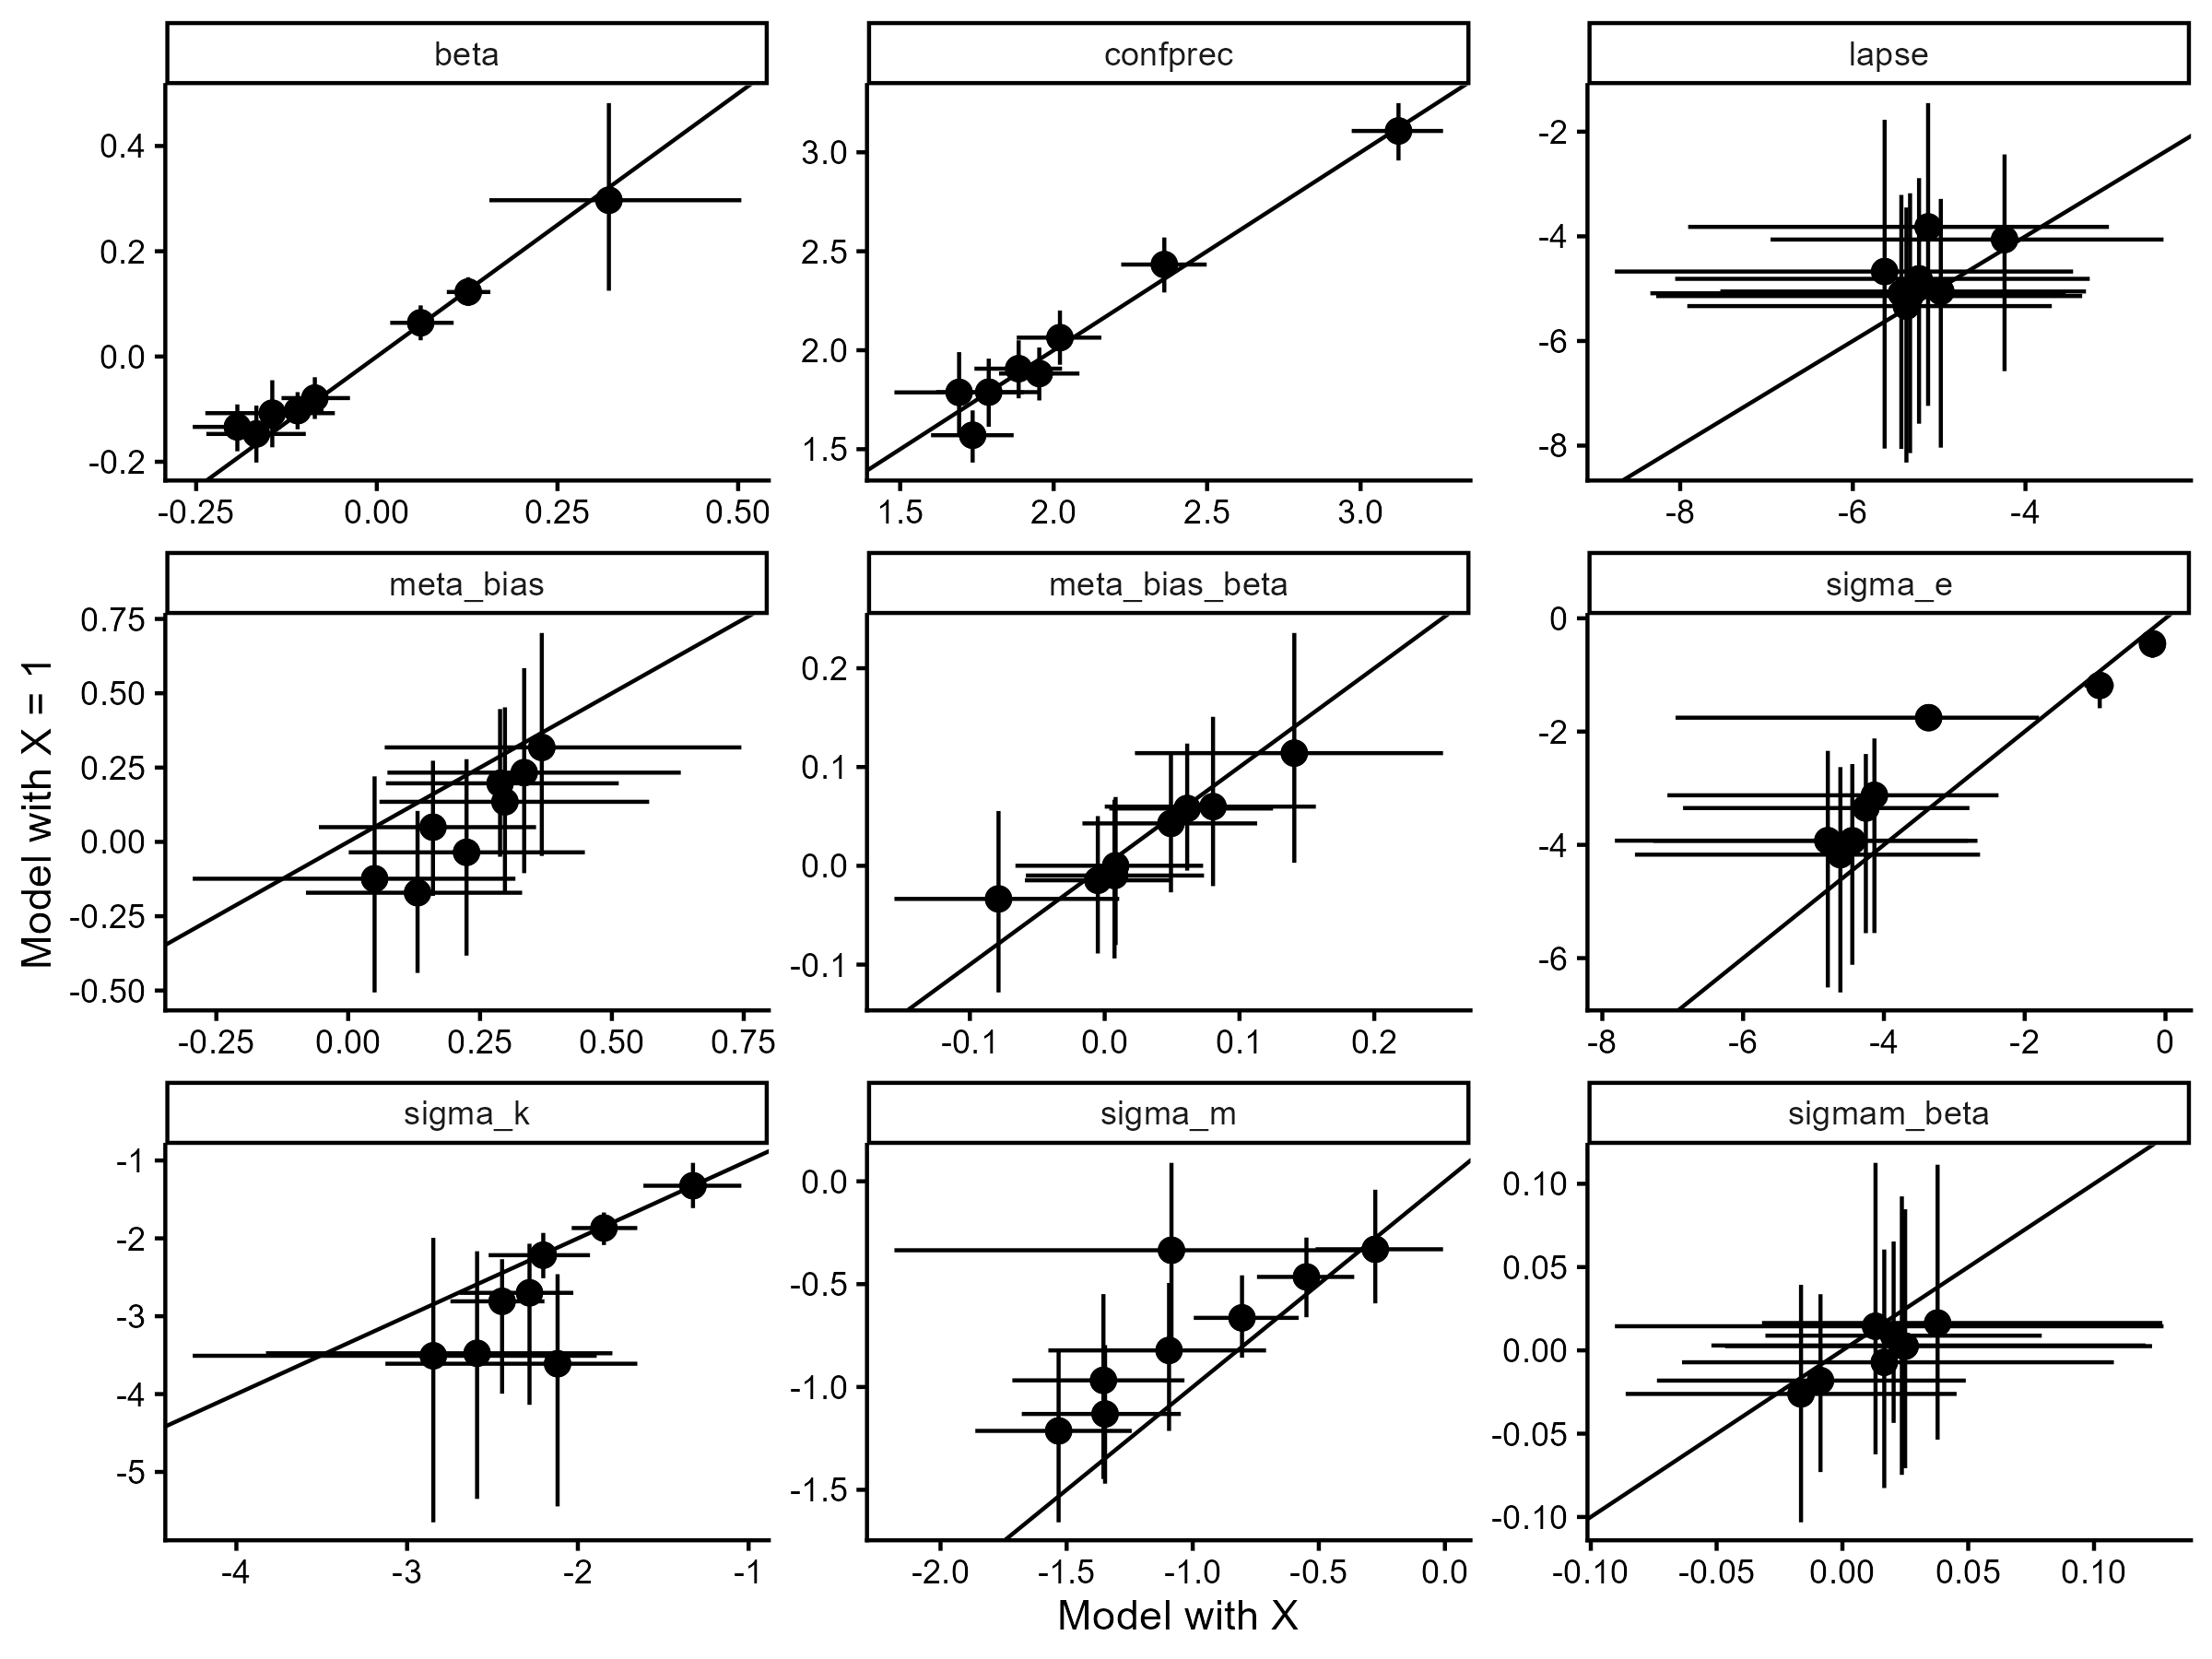
\includegraphics[width=6in,height=4.5in]{../Figures/parameter_comparison_plot} \end{center}

The two models align well in their subject-level parameter estimates,
further justifying this theoretically motivated simplification.

\subsubsection{Posterior predictive
checks}\label{posterior-predictive-checks}

Next, we show posterior predictive checks of the hierarchical heuristic
model for our pilot participants.

\begin{center}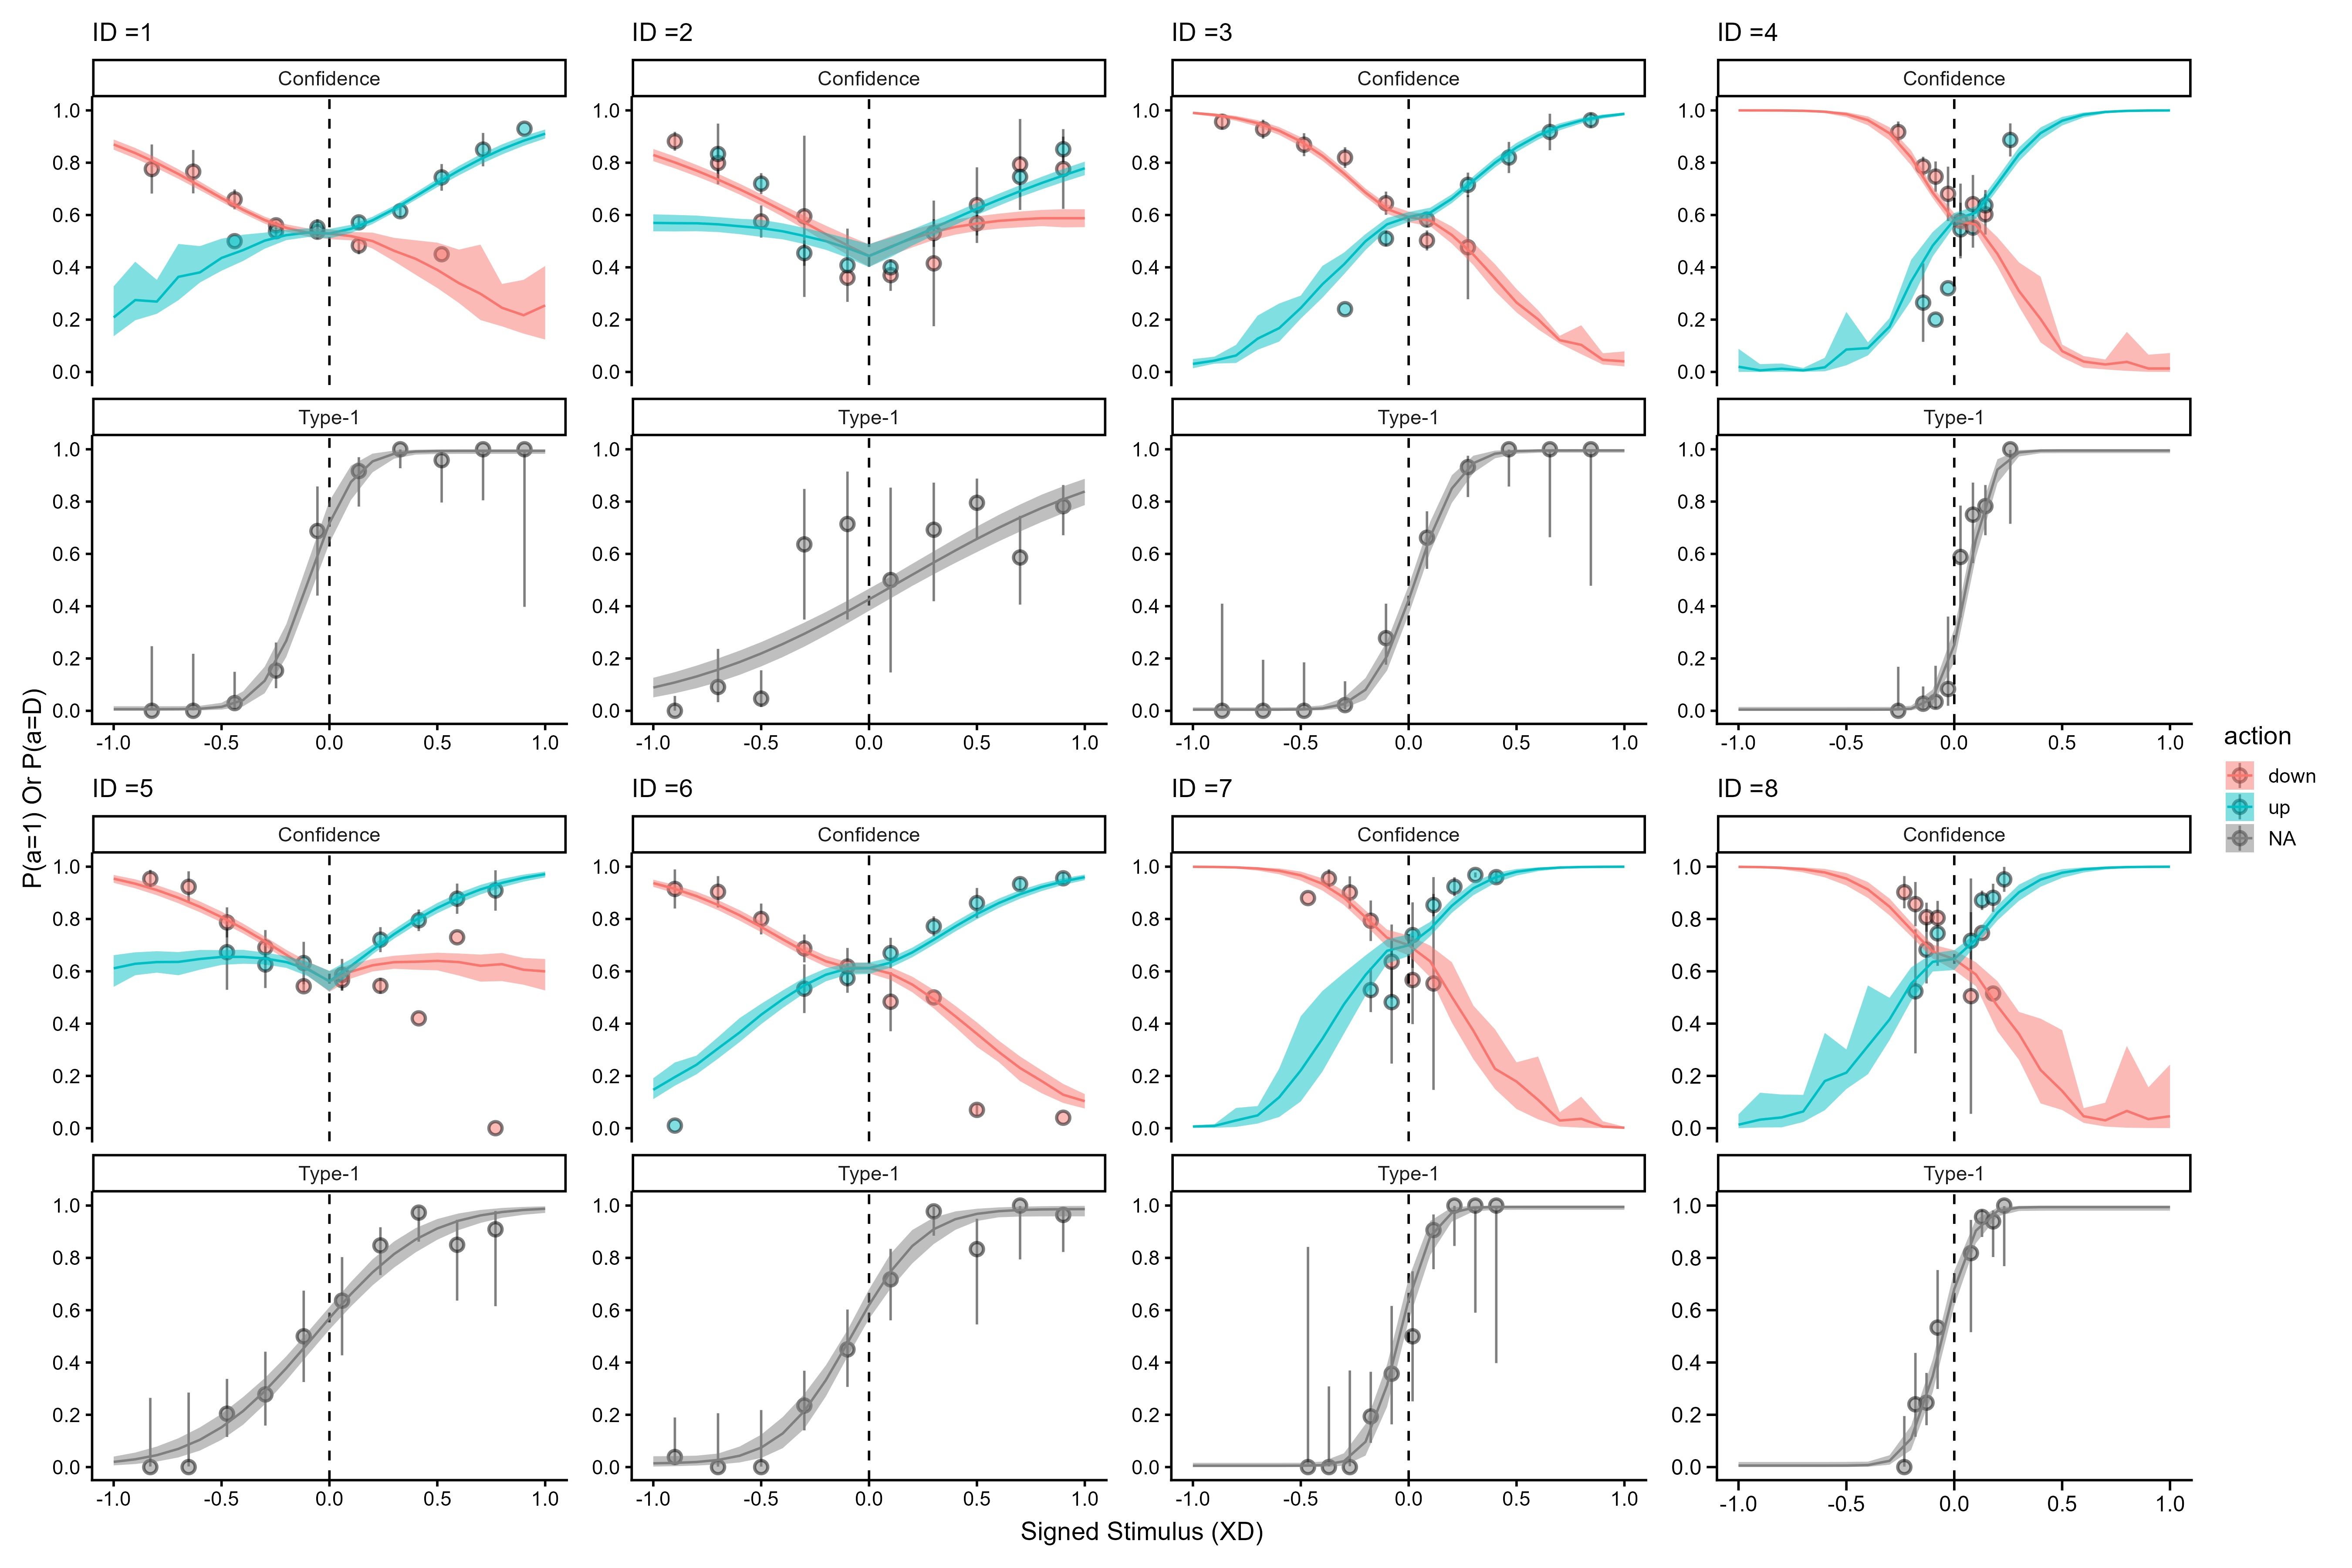
\includegraphics[width=6in,height=4.5in]{../Figures/Pilot_predictive_checks} \end{center}

\subsubsection{Hierarchical parameter
recovery}\label{hierarchical-parameter-recovery}

To further assess the robustness of our model implementation and the
planned sequential sampling procedure, we simulated new participants
from the posterior distribution of the hierarchical model. We extracted
a single posterior draw and simulated 25 participants from it, then
fitted the model to increasing numbers of participants (5, 7, 9, 12, 15,
20, 25) to demonstrate that the sequential sampling approach is
feasible. This also allowed us to perform parameter recovery on the
hierarchical model without additional computational resources. Below, we
show that the model adequately recovers its parameters at both the
subject and group level for parameters of interest.

\begin{center}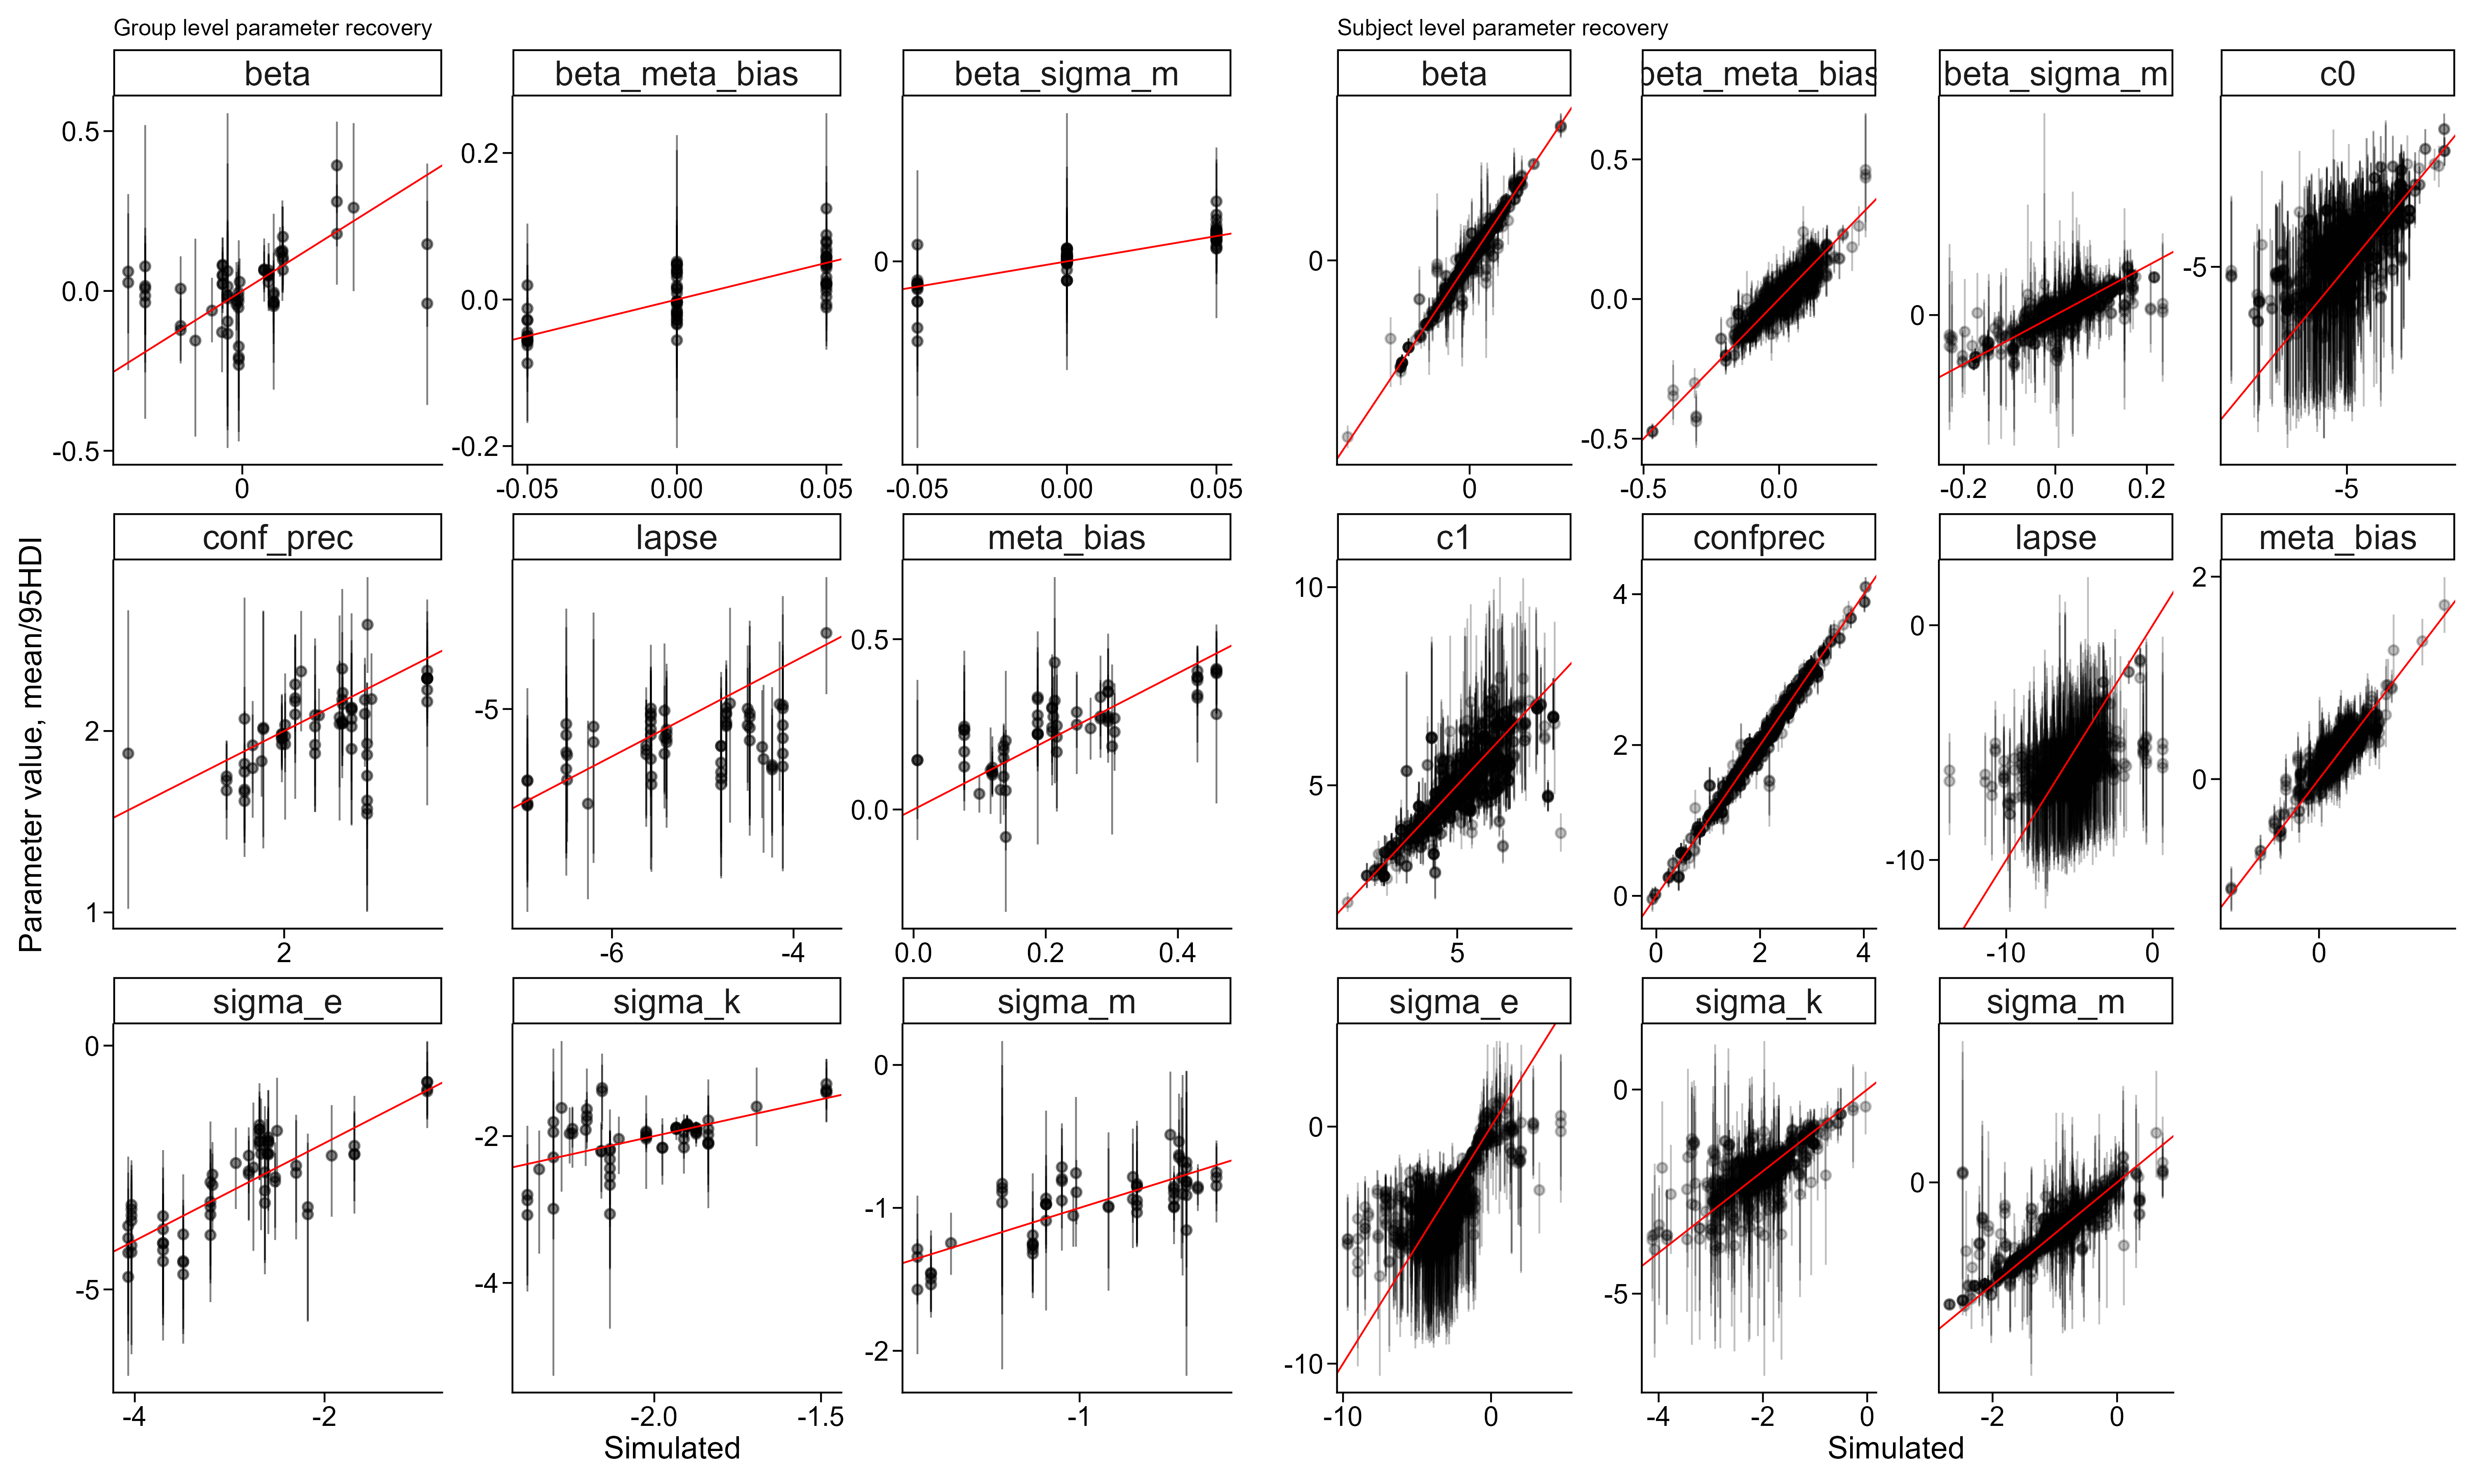
\includegraphics[width=6.5in,height=4.875in]{../Figures/parameterrecovery_hier} \end{center}

\subsubsection{Sequential sampling}\label{sequential-sampling}

\paragraph{Priors}\label{priors}

Because our sequential sampling approach uses Bayes factors for the
termination of data collection, the prior distributions are highly
influential. For transparency, we visualize the curves permitted by the
prior below. Interested readers are also referred to the
\href{../Sequential\%20sampling/}{Sequential Sampling} directory, which
contains scripts for fitting, visualizing, and diagnosing our model.

\begin{center}
\includegraphics{Pre-registration_files/figure-latex/unnamed-chunk-24-1} \end{center}

The plot above shows prior predictive checks of the group-level
parameters (i.e., these curves represent group-level predictions). The
curves span a wide range of possible patterns. To test whether our
sequential sampling approach works, we simulate data from draws of the
posterior distribution of our pilot data and examine how the Bayes
factors for both hypotheses evolve as more participants are collected.
Rather than using posterior draws of the parameters of interest
(\(\mu_{\Delta{\sigma_{m_s}}}\) and \(\mu_{\Delta{\mu_{\beta_c}}}\)), we
fixed these to \(-0.05\), \(0\), or \(0.05\) to test whether we can
detect effects of this magnitude in both directions and also terminate
sampling when the effect is zero. Below, we display the size of these
effects (simulated from the mean of the group means).

\begin{center}
\includegraphics{Pre-registration_files/figure-latex/unnamed-chunk-25-1} \end{center}

As described above, we simulated participants from draws of the
posterior informed by our pilot data. We then fitted the model to
increasing numbers of participants (5, 7, 9, 12, 15, 20, 25) to
demonstrate the feasibility of the sequential sampling approach. Below,
we show five such trajectories of Bayes factors as a function of sample
size, alongside a panel showing how the posterior distribution of the
parameter of interest changes with increasing sample size.

\begin{center}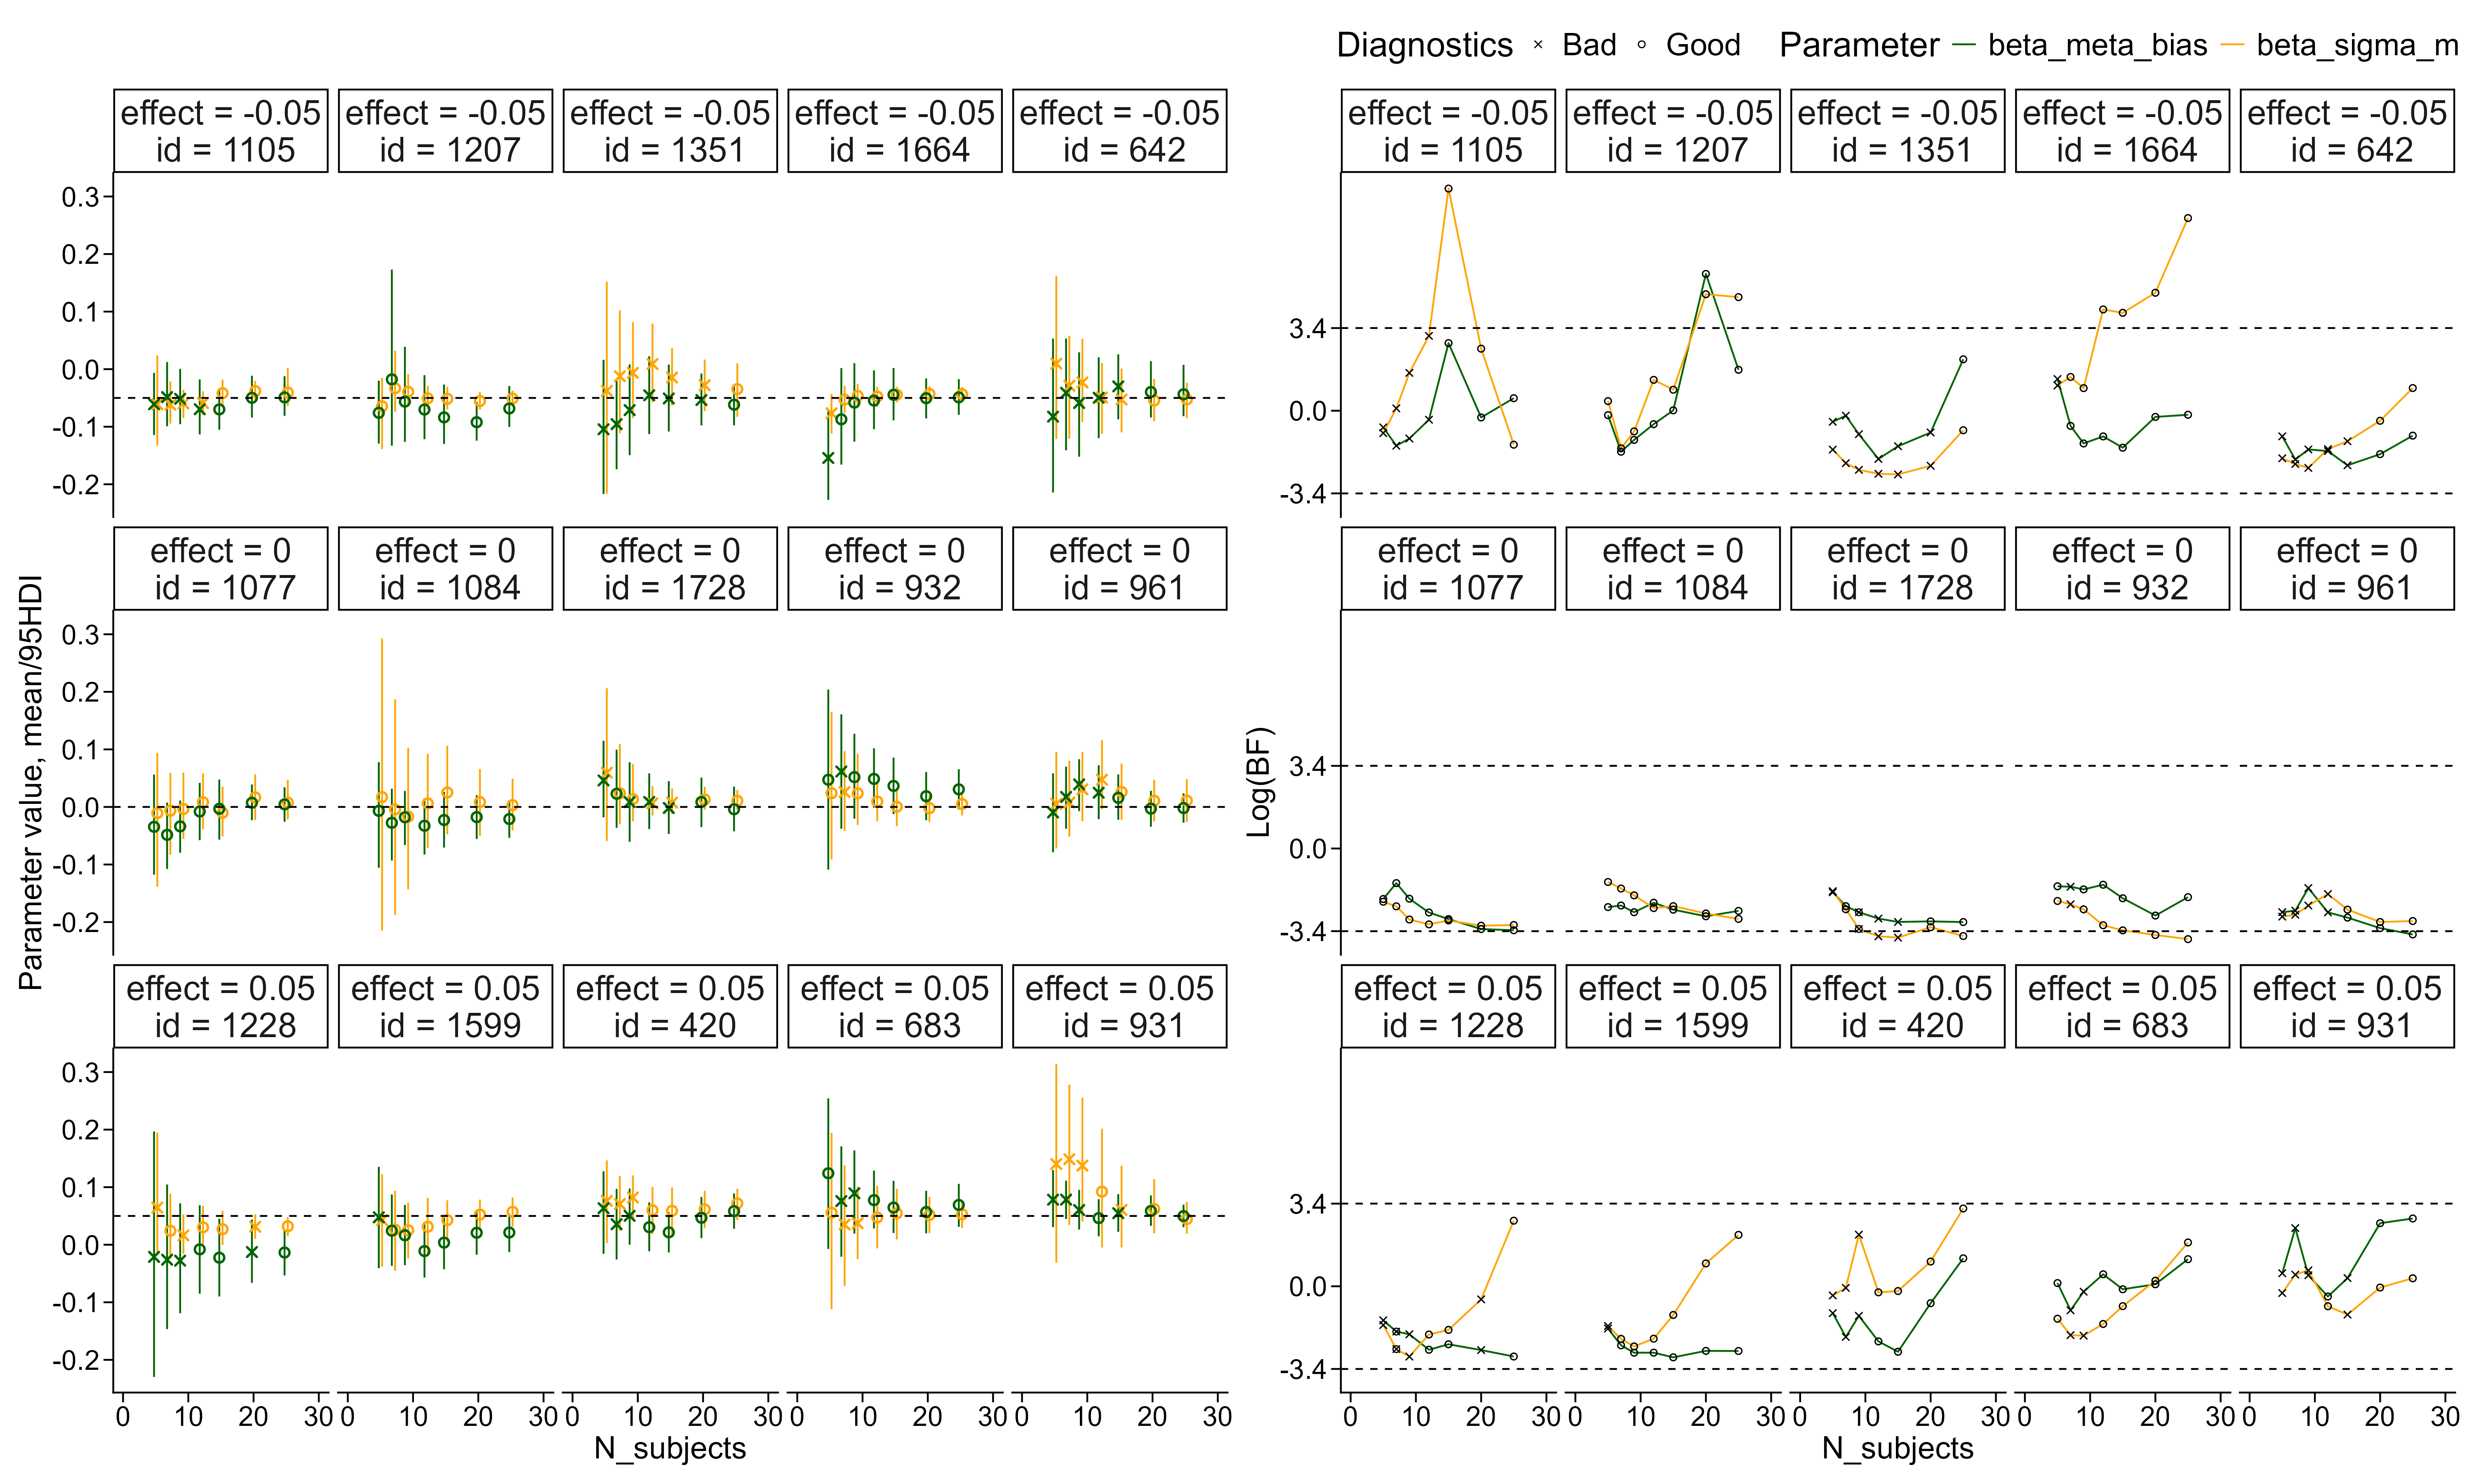
\includegraphics[width=6.5in,height=4.333in]{../Figures/sequential_samping_plot} \end{center}

The above plot shows how the estimated effect of the interval between
choice and confidence rating evolves for both metacognitive bias (green)
and metacognitive noise (orange). Circles indicate fitted models without
divergences, with effective sample sizes above 400 for both bulk and
tails and \(\hat{R}\) values below 1.03. The left panel displays the
posterior distribution of each parameter for increasing sample sizes.
The right panel displays the corresponding Bayes factors for the same
posterior draws fitted to our pilot data.

The above plot also shows that convergence issues may arise even with
this model. Below, we describe our approach for identifying and handling
convergence issues.

We will collect data from 15 participants before fitting the
hierarchical model for the first time and testing the Bayes factor,
because hierarchical models generally require a minimum amount of data
to converge (see also the simulation above). After this initial fit, we
will check the Bayes factor after each additional 5 participants, which
coincides with the expected number of participants collected per day.

\begin{center}\rule{0.5\linewidth}{0.5pt}\end{center}

\section{Part 3: Design, Methods, and
Hypotheses}\label{part-3-design-methods-and-hypotheses}

\subsection{Experimental study}\label{experimental-study}

This study examines motion discrimination and metacognition in a Random
Dot Motion (RDM) task. Specifically, we ask whether the time between a
first-order choice and a confidence judgements (post-decisional time)
influences metacognitive uncertainty. We operationalize this as whether
confidence ratings track the probability of being correct more closely
when participants are required to wait longer before giving their
confidence ratings, than when they can respond immediately

Dynamic models of metacognition assume that evidence is accumulated
until a response boundary is reached and a binary decision is initiated.
After the binary choice, additional evidence is assumed to be
accumulated post-decisionally to inform the confidence rating. If this
post-decisional evidence accumulation is informative about the
correctness of the choice, increasing the post-decisional time window
should improve the quality of the confidence ratings. This improvement
would be shown as confidence ratings more closely approximating the
objective probability that the choice was correct. However, if the
evidence used for the confidence rating is already fully computed around
the time of the decision (i.e., pre-decisionally), one would expect no
difference, or even the opposite effect. Confidence ratings becoming
less consistent with the probability of being correct would indicate
that some information leakage is taking place, perhaps due to memory
constraints. In this study, we manipulate the post-decisional time
window to examine its effects on the quality of confidence ratings.
Previous studies of post-decisional evidence accumulation have generally
found that such accumulation is easiest to detect in speeded
decision-making tasks, particularly on easy trials, where increased
post-decisional time can decrease confidence ratings for incorrect
choices.

In this study, we use a non-speeded perceptual decision-making task with
individually calibrated difficulty levels ranging from very easy to very
hard. We test whether post-decisional evidence accumulation can unfold
over a longer time period even in non-speeded tasks. Because previous
literature on this question is inconclusive, we adopt a Bayesian
sequential-sampling framework. This approach allows us to quantify
evidence for the null hypothesis (that post-decisional time does not
change the quality of confidence ratings) and to collect only the number
of participants necessary to reach a decision threshold.

\subsubsection{Computational model}\label{computational-model}

To test whether the post-decisional response window changes how
informative confidence ratings are about choice correctness, we
constructed a hierarchical Bayesian model grounded in signal detection
theory and motor control theory. The model assumes that agents exhibit
variability both in the encoding of the physical stimulus, as in
traditional signal detection theory, and in the selection of a choice
given the internal evidence. Consistent with motor control theories, the
model assumes that an efference copy is generated before the efferent
signal is sent to the acting limb. This efference copy is corrupted by
additional noise, consistent with other generative metacognition models,
before being combined with the executed action to compute confidence in
the chosen response. The model accounts for error monitoring through the
inclusion of choice variability. For the full derivation and
simulations, see the previous page. Here it suffices to note that the
metacognitive uncertainty parameter \(\sigma_m\) governs the
relationship between confidence ratings and choice correctness, as
\(\sigma_m\) increases, confidence becomes less informative about
whether the choice was correct.

\subsubsection{Hypotheses}\label{hypotheses}

\begin{enumerate}
\def\labelenumi{\arabic{enumi}.}
\item
  \textbf{Hypothesis 1:} Increasing the post-decisional time window will
  lead to no improvement in the relationship between confidence and
  accuracy.

  \begin{itemize}
  \tightlist
  \item
    \textbf{Test specification:}\\
    This hypothesis is tested by allowing the metacognitive uncertainty
    (\(\sigma_m\)) parameter to vary linearly on the log scale with the
    post-decisional time window. Because this is the main parameter of
    interest, we will sequentially test whether the Bayes factor for
    this parameter has reached our termination criteria of either 30 or
    1/30.
  \end{itemize}
\item
  \textbf{Hypothesis 2:} Increasing the post-decisional time window will
  lead to no difference in confidence bias.

  \begin{itemize}
  \tightlist
  \item
    \textbf{Test specification:}\\
    This hypothesis is tested by allowing the \(mu_{\beta_c}\) parameter
    to vary by post-decisional time window. The primary test evaluates
    whether the group-level parameter differs from 0 (i.e., whether the
    95\% highest density interval includes 0). We also aim to report the
    Bayes factor to quantify the strength of the evidence relative to
    the null (i.e., there is no difference). This test will be conducted
    when the data collection has been terminated.
  \end{itemize}
\end{enumerate}

\subsubsection{Priors and Sequential
Sampling.}\label{priors-and-sequential-sampling.}

To limit the number of participants needed to obtain sufficient
evidence, we will use a sequential-sampling design. Recruitment will be
terminated when the Bayes factor described above reaches either 30 or
1/30, or when 50 non-excluded participants have been collected. We will
begin examining the Bayes factor in increments of 5 participants once 15
non-excluded participants have been reached (see exclusion criteria).
This minimum of 15 is set to ensure stability of the model estimates;
the increment of 5 reflects our expected daily testing rate. The Bayes
factor used in this study is the Savage-Dickey density ratio evaluated
at 0
(\citeproc{ref-WAGENMAKERSBayesianHypothesisTestingPsychologistsTutorialSavage2010a}{Wagenmakers
et al. 2010}).

Below we define the initial sampler parameters, the convergence
diagnostics we require, and contingency plans if the sampler does not
converge.

\paragraph{Initial Sampler
Configuration}\label{initial-sampler-configuration}

The model is initially estimated using the following sampler settings:

\begin{itemize}
\tightlist
\item
  Number of chains: 4\\
\item
  Number of iterations per chain: 1000\\
\item
  Warmup iterations: 1000
\item
  Target acceptance rate (\texttt{adapt\_delta}): 0.95\\
\item
  Maximum tree depth (\texttt{max\_treedepth}): 12
\end{itemize}

These values represent our baseline configuration for model estimation.

\subparagraph{Convergence Criteria}\label{convergence-criteria}

Sampler convergence and reliability will be assessed using the following
diagnostics:

\begin{itemize}
\tightlist
\item
  \(\hat{R}\) values below 1.03 for all group level parameters\\
\item
  Effective sample size (ESS) above 400 for all group level parameters\\
\item
  Zero divergent transitions after warmup\\
\item
  No saturation of the maximum tree depth\\
\item
  Well-mixing trace plots
\end{itemize}

If these criteria are met, the sampling procedure will be considered
satisfactory.

\subparagraph{Contingency Procedures}\label{contingency-procedures}

If the above convergence criteria are not met, we will apply the
following steps depending on the convergence failure:

\begin{itemize}
\tightlist
\item
  Increase the number of iterations.
\item
  Increase the target acceptance rate (\texttt{adapt\_delta}).
\item
  Increase the maximum tree depth (\texttt{max\_treedepth}).
\item
  Reconsider model parameterization (i.e.~centered vs non-centered
  parameterization).
\item
  Estimate the lapse-rate parameter non-hierarchically
\item
  Estimate the choice variability parameter non-hierarchically
\end{itemize}

These steps are intended to improve sampler stability and ensure
reliable posterior estimation.

The full Stan model and the scripts for checking diagnostics and model
fit are available in the sequential-sampling directory
(\texttt{../Sequential\ Sampling}).

\subsection{Participants}\label{participants}

Eligible participants will be 18--40 years old, have normal or
corrected-to-normal vision, and be proficient in English. Individuals
with neurological or psychiatric diagnoses, or those taking medication
that may affect cognitive performance, will not be eligible.
Participants will be recruited through COBE Lab's participant pool to
ensure fast and effective recruitment and will be compensated 110 DKK.

\subsection{Design}\label{design}

This study consists of a single lab visit of an hour, where participants
perform a computer experiment. Stimulus were presented on a 64x39xm
monitor (2560x1440 resolution, 60 Hz refresh rate) at a viewing distance
of 60 cm. The monitor was calibrated to RGB color space. Stimulus
presentation was controlled using PsychoPy with synchronization to the
Eyelink 1000
(\citeproc{ref-PEIRCEPsychoPy2ExperimentsBehaviorMadeEasy2019}{Peirce et
al. 2019}). The experiment uses a random dot motion (RDM)
decision‑making task. On each trial, participants view a random dot
kinematogram in which a proportion of dots move coherently upward or
downward. While the dots are displayed, participants indicate whether
the overall motion is `up' or `down' by pressing a corresponding key.
The dots remained on the screen for at most 2 seconds or when the
participant responded, trials without a response within this window are
classified as no‑response trials. After indicating their response,
participants view a post‑decisional fixation cross. The duration of this
interval is the main experimental manipulation and is randomly drawn
from a uniform distribution ranging from 2 to 5 seconds
(\(PostD_i \sim \text{U}(2, 5)\)). After the interval, participants
provide a metacognitive evaluation of their decision. They are asked,
`How confident were you in your decision?' and respond using a visual
analogue scale ranging from `certainly wrong' to `certainly right.'
Participants navigate the scale using the arrow keys and confirm their
response with a key press. If no response is made within 3 seconds, the
trial is classified as a no‑response trial. Before the start of each new
trial, an inter‑trial interval is presented consisting of a fixation
cross. The duration of this interval is drawn from a log‑normal
distribution with a mean of 1 second and a standard deviation of 0.1
(\(ITI_i \sim \text{Lognormal}(1,0.1)\)).

In total, participants will complete 288 trials, spread over 8 blocks of
36 trials. Pilot data indicated that this trial count was sufficient for
good subject-level-parameter estimation. Before the main experiment
begins, participants receive instructions on how to perform the decision
task. They then complete six easy, non‑speeded practice trials without
confidence ratings, followed by 120 more difficult practice trials.
Afterward, participants receive additional instructions about the
confidence scale and complete 10 easy, non‑speeded practice trials that
include confidence ratings, after which the main experiment begins. The
key variables of interest are response choice, accuracy, response time,
confidence rating, and the response time associated with those
confidence rating.

To ensure that task difficulty is calibrated at the individual level,
the 120 harder practice trials serve as a staircase procedure. In a
random dot kinematogram, task difficulty is determined by several
stimulus properties, that can be broadly grouped into two categories:
stimulus parameters and stimulus noisiness. To ensure that difficulty is
optimally calibrated for each participant, we use the first 40 of the
harder practice trials to staircase the dotlife parameter in the
Dotstimclass in
\href{https://www.psychopy.org/api/visual/dotstim.html}{psychopy}. This
parameter determines how many frames a dot persists before disappearing.
Once an appropriate dot‑life value is identified, we begin staircasing
coherence. Coherence controls the stimulus signal-to-noise ratio and is
the most commonly manipulated difficulty parameter in the literature. It
ranges from 0 to 1 and determines the proportion of signal to noise
dots, with higher values indicating a greater proportion of signal dots.

The remaining 80 trials are used to estimate the slope and threshold of
the participant's psychometric function on coherence. Both staircases
are implemented in PsychoPy using the QUEST+ Bayesian adaptive
procedure, which selects each stimulus to minimize posterior entropy
over the psychometric parameters
(\citeproc{ref-WATSONQUESTGeneralMultidimensionalBayesianAdaptivePsychometric2017}{Watson
2017}). Using the estimated psychometric function, we determine the
coherence levels for the main experiment based on a set of predefined
target accuracies (\(ACC = [0.51, 0.6, 0.7, 0.8, 0.99]\)). The
corresponding coherence values are then sampled in a quasi‑normal
fashion: the extreme accuracy levels (0.51 and 0.99) appear once per
direction, the intermediate levels appear twice, and the 0.70 level
appears three times. In each block of the main experiment, trials are
presented in a pseudo‑randomized sequence of upward and downward motion
such that no more than three consecutive trials share the same
direction. This reduces the risk of implicit directional bias. Together,
these procedures ensure that participants use the full confidence scale
and that difficulty is balanced across upward and downward motion
directions.

\subsection{Exclusion criteria}\label{exclusion-criteria}

Because the task is a two‑alternative forced‑choice decision, chance
performance is 50\%. For each participant, we will compute overall
accuracy across all main‑task trials and will exclude all participants
with an accuracy lower than 60\%. For our trial count, accuracy below
this threshold is not reliably above chance under a binomial model of
guessing. Furthermore, given the stimulus calibration procedure, an
optimal observer is expected to achieve approximately 71\% accuracy.
Accuracy below 60\% is therefore inconsistent with meaningful task
engagement.

Additionally, trials with a response time below 150 ms will be coded as
no response trials and excluded from further analysis, as responses this
fast are unlikely to reflect genuine perceptual processing. Participants
with a no-response rate greater than 30\% (combining decision,
confidence responses and response times below 150 ms), will be excluded,
as a high proportion of missed responses also indicates insufficient
engagement with the task.

\subsection{Physiological measures}\label{physiological-measures}

As an additional data stream we also collect physiological measures from
each participant Specifically, we record eyetracking (including pupil
size) using an Eyelink 1000, furthermore we will collect
electrocardiogram (ECG) and respiration measures using Biopac Systems
(\citeproc{ref-DataAcquisitionLoggersAmplifiersTransducersElectrodes}{BIOPAC
Systems, Inc., n.d.}). To ensure accurate eye-tracking calibration, the
experimental script performs recalibration after each block, which also
provides participants with regular breaks.

These physiological measures will allow us to test the theoretical
assumptions of our model of confidence ratings using physiological data.
In particular, we will investigate whether autonomic responses reflect
the agent's appraisal of their own action. We expect that an initial
physiological response will occur following stimulus presentation
corresponding to the orienting response
(\citeproc{ref-GABAYOrientingAttentionPupilSizeNorepinephrineSystem2011}{Gabay
et al. 2011}). Crucially, we predict a second response of the
physiological measures, shortly after the initial decision. This
physiological response is expected to unfold within a time window of
approximately 500--2500 ms after the initial response, corresponding to
the period during which the action is being appraised (note the general
sluggishness of the autonomic signals making this range wide).
Importantly, this physiological response is expected to occur before the
explicit presentation of the confidence rating, which would indicate
that the appraisal process and computation of confidence begin prior to
the overt confidence response. Additionally, we expect the initial
response to the stimulus to be conditional on the stimulus intensity,
such that higher coherence leads to larger amplitudes of the
physiological responses. We further believe that the second
physiological response, the appraisal of the action, will be conditional
on the internal prediction error between the expected evidence
distribution and the observed action, quantified by the internal
prediction error \(S_i\). This quantity is largest for errors at high
stimulus intensity and decreases toward threshold, while for correct
responses it is largest near threshold and decays to zero at high
stimulus intensity. These predictions are directly derivable from the
model and generate two dissociable physiological signatures: a
stimulus-locked response scaling with \textbar XD\textbar{} that should
be independent of the action and choice accuracy, and an action-locked
response scaling with \(S_i\) which diverges by accuracy as stimulus
intensity increases.

\subsubsection{Physiological analyses}\label{physiological-analyses}

\begin{enumerate}
\def\labelenumi{\arabic{enumi}.}
\item
  \textbf{Physiological-Hypothesis 1:} Autonomic responses, particularly
  pupil size, will show an initial response to the stimulus, but also a
  second response after the decision, reflecting action appraisal.
\item
  \textbf{Physiological-Hypothesis 2:} The Autonomic responses for the
  initial response to the stimulus will scale with the stimulus
  intensity, whereas the second response will scale with the internal
  prediction error \(S_i\). Which predicts the greatest response for
  high stimulus intensity incorrect choices, an intermediate response
  near threshold regardless of accuracy, and the smallest response for
  high stimulus intensity correct choices.
\end{enumerate}

As the analysis plans for these two hypotheses are not fully developed,
and do not depend on the sequential sampling, we designate them as
exploratory.

\begin{center}\rule{0.5\linewidth}{0.5pt}\end{center}

\section{References}\label{references}

\phantomsection\label{refs}
\begin{CSLReferences}{1}{1}
\bibitem[\citeproctext]{ref-BARANSKIProbingLocusConfidenceJudgmentsExperimentsTime1998}
Baranski, J. V., and W. M. Petrusic. 1998. {``Probing the Locus of
Confidence Judgments: Experiments on the Time to Determine
Confidence.''} \emph{Journal of Experimental Psychology. Human
Perception and Performance} 24 (3): 929--45.
\url{https://doi.org/10.1037//0096-1523.24.3.929}.

\bibitem[\citeproctext]{ref-BARANSKITestingArchitecturesDecisionconfidenceRelation2001}
Baranski, J. V., and W. M. Petrusic. 2001. {``Testing Architectures of
the Decision-Confidence Relation.''} \emph{Canadian Journal of
Experimental Psychology = Revue Canadienne De Psychologie Experimentale}
55 (3): 195--206. \url{https://doi.org/10.1037/h0087366}.

\bibitem[\citeproctext]{ref-DataAcquisitionLoggersAmplifiersTransducersElectrodes}
BIOPAC Systems, Inc. n.d. {``Data {Acquisition}, {Loggers},
{Amplifiers}, {Transducers}, {Electrodes} \textbar{} {BIOPAC}.''}
Accessed March 12, 2026. \url{https://www.biopac.com/}.

\bibitem[\citeproctext]{ref-CAZIOTPerceptualConfidenceJudgmentsReflectSelfconsistency2021}
Caziot, Baptiste, and Pascal Mamassian. 2021. {``Perceptual Confidence
Judgments Reflect Self-Consistency.''} \emph{Journal of Vision} 21 (12):
8. \url{https://doi.org/10.1167/jov.21.12.8}.

\bibitem[\citeproctext]{ref-DESENDERUnderstandingNeuralSignalsPostdecisionalPerformanceMonitoring2021}
Desender, Kobe, K. Richard Ridderinkhof, and Peter R. Murphy. 2021.
{``Understanding Neural Signals of Post-Decisional Performance
Monitoring: {An} Integrative Review.''} \emph{eLife} 10 (August):
e67556. \url{https://doi.org/10.7554/eLife.67556}.

\bibitem[\citeproctext]{ref-FLEMINGHMetadHierarchicalBayesianEstimationMetacognitiveEfficiency2017}
Fleming, Stephen M. 2017. {``{HMeta-d}: Hierarchical {Bayesian}
Estimation of Metacognitive Efficiency from Confidence Ratings.''}
\emph{Neuroscience of Consciousness} 2017 (1): nix007.
\url{https://doi.org/10.1093/nc/nix007}.

\bibitem[\citeproctext]{ref-FLEMINGSelfEvaluationDecisionMakingGeneralBayesianFrameworkMetacognitive2017}
Fleming, Stephen M., and Nathaniel D. Daw. 2017. {``Self-{Evaluation} of
{Decision-Making}: {A General Bayesian Framework} for {Metacognitive
Computation}.''} \emph{Psychological Review} 124 (1): 91--114.
\url{https://doi.org/10.1037/rev0000045}.

\bibitem[\citeproctext]{ref-FLEMINGNeuralMediatorsChangesMindPerceptualDecisions2018a}
Fleming, Stephen M., Elisabeth J. van der Putten, and Nathaniel D. Daw.
2018. {``Neural Mediators of Changes of Mind about Perceptual
Decisions.''} \emph{Nature Neuroscience} 21 (4): 617--24.
\url{https://doi.org/10.1038/s41593-018-0104-6}.

\bibitem[\citeproctext]{ref-FUNGSimilaritiesDifferencesEffectsDifferentStimulusManipulations2025}
Fung, Herrick, Medha Shekhar, Kai Xue, Manuel Rausch, and Dobromir
Rahnev. 2025. {``Similarities and Differences in the Effects of
Different Stimulus Manipulations on Accuracy and Confidence.''}
\emph{Consciousness and Cognition} 136 (November): 103942.
\url{https://doi.org/10.1016/j.concog.2025.103942}.

\bibitem[\citeproctext]{ref-GABAYOrientingAttentionPupilSizeNorepinephrineSystem2011}
Gabay, Shai, Yoni Pertzov, and Avishai Henik. 2011. {``Orienting of
Attention, Pupil Size, and the Norepinephrine System.''}
\emph{Attention, Perception, \& Psychophysics} 73 (1): 123--29.
\url{https://doi.org/10.3758/s13414-010-0015-4}.

\bibitem[\citeproctext]{ref-GOUEYTESEvidenceAccumulationPresupplementaryMotorAreaInsula2025}
Goueytes, Dorian, François Stockart, Alexis Robin, et al. 2025.
{``Evidence Accumulation in the Pre-Supplementary Motor Area and Insula
Drives Confidence and Changes of Mind.''} \emph{Nature Communications}
16 (1): 6998. \url{https://doi.org/10.1038/s41467-025-61744-8}.

\bibitem[\citeproctext]{ref-HANGYAMathematicalFrameworkStatisticalDecisionConfidence2016}
Hangya, Balázs, Joshua I. Sanders, and Adam Kepecs. 2016. {``A
{Mathematical Framework} for {Statistical Decision Confidence}.''}
\emph{Neural Computation} 28 (9): 1840--58.
\url{https://doi.org/10.1162/NECO_a_00864}.

\bibitem[\citeproctext]{ref-KIANIRepresentationConfidenceAssociatedDecisionNeuronsParietal2009}
Kiani, Roozbeh, and Michael N. Shadlen. 2009. {``Representation of
{Confidence Associated} with a {Decision} by {Neurons} in the {Parietal
Cortex}.''} \emph{Science} 324 (5928): 759--64.
\url{https://doi.org/10.1126/science.1169405}.

\bibitem[\citeproctext]{ref-KUBINECOrderedBetaRegressionParsimoniousWellFittingModel2023}
Kubinec, Robert. 2023. {``Ordered {Beta Regression}: {A Parsimonious},
{Well-Fitting Model} for {Continuous Data} with {Lower} and {Upper
Bounds}.''} \emph{Political Analysis} 31 (4): 519--36.
\url{https://doi.org/10.1017/pan.2022.20}.

\bibitem[\citeproctext]{ref-MANISCALCOSignalDetectionTheoreticApproachEstimatingMetacognitive2012}
Maniscalco, Brian, and Hakwan Lau. 2012. {``A Signal Detection Theoretic
Approach for Estimating Metacognitive Sensitivity from Confidence
Ratings.''} \emph{Consciousness and Cognition}, Beyond the {Comparator
Model}, vol. 21 (1): 422--30.
\url{https://doi.org/10.1016/j.concog.2011.09.021}.

\bibitem[\citeproctext]{ref-MIHALIIntrospectiveInferenceCounteractsPerceptualDistortion2023a}
Mihali, Andra, Marianne Broeker, Florian D. M. Ragalmuto, and Guillermo
Horga. 2023. {``Introspective Inference Counteracts Perceptual
Distortion.''} \emph{Nature Communications} 14 (1): 7826.
\url{https://doi.org/10.1038/s41467-023-42813-2}.

\bibitem[\citeproctext]{ref-NAVAJASIdiosyncraticNatureConfidence2017}
Navajas, Joaquin, Chandni Hindocha, Hebah Foda, Mehdi Keramati, Peter E.
Latham, and Bahador Bahrami. 2017. {``The Idiosyncratic Nature of
Confidence.''} \emph{Nature Human Behaviour} 1 (11): 810--18.
\url{https://doi.org/10.1038/s41562-017-0215-1}.

\bibitem[\citeproctext]{ref-OZTELMetricErrorMonitoringComponentMetacognitiveProcessing2024}
Öztel, Tutku, and Fuat Balcı. 2024. {``Metric Error Monitoring as a
Component of Metacognitive Processing.''} \emph{European Journal of
Neuroscience} 59 (5): 807--21. \url{https://doi.org/10.1111/ejn.16182}.

\bibitem[\citeproctext]{ref-PEIRCEPsychoPy2ExperimentsBehaviorMadeEasy2019}
Peirce, Jonathan, Jeremy R. Gray, Sol Simpson, et al. 2019.
{``{PsychoPy2}: {Experiments} in Behavior Made Easy.''} \emph{Behavior
Research Methods} 51 (1): 195--203.
\url{https://doi.org/10.3758/s13428-018-01193-y}.

\bibitem[\citeproctext]{ref-PETRUSICJudgingConfidenceInfluencesDecisionProcessingComparative2003}
Petrusic, William M., and Joseph V. Baranski. 2003. {``Judging
Confidence Influences Decision Processing in Comparative Judgments.''}
\emph{Psychonomic Bulletin \& Review} 10 (1): 177--83.
\url{https://doi.org/10.3758/BF03196482}.

\bibitem[\citeproctext]{ref-PLESKACTwostageDynamicSignalDetectionTheoryChoice2010}
Pleskac, Timothy J., and Jerome R. Busemeyer. 2010. {``Two-Stage Dynamic
Signal Detection: {A} Theory of Choice, Decision Time, and
Confidence.''} \emph{Psychological Review} (US) 117 (3): 864--901.
\url{https://doi.org/10.1037/a0019737}.

\bibitem[\citeproctext]{ref-RAUSCHFoldedXpatternNotNecessarilyStatisticalSignature2019}
Rausch, Manuel, and Michael Zehetleitner. 2019. {``The Folded
{X-pattern} Is Not Necessarily a Statistical Signature of Decision
Confidence.''} \emph{PLOS Computational Biology} 15 (10): e1007456.
\url{https://doi.org/10.1371/journal.pcbi.1007456}.

\bibitem[\citeproctext]{ref-RESULAJChangesMindDecisionmaking2009}
Resulaj, Arbora, Roozbeh Kiani, Daniel M. Wolpert, and Michael N.
Shadlen. 2009. {``Changes of Mind in Decision-Making.''} \emph{Nature}
461 (7261): 263--66. \url{https://doi.org/10.1038/nature08275}.

\bibitem[\citeproctext]{ref-SANCHEZ-FUENZALIDAConfidenceReportsPerceptualDecisionMakingDissociate2025}
Sánchez-Fuenzalida, Nicolás, Simon van Gaal, Stephen M. Fleming, Julia
M. Haaf, and Johannes J. Fahrenfort. 2025. {``Confidence Reports During
Perceptual Decision Making Dissociate from Changes in Subjective
Experience.''} \emph{Communications Psychology} 3 (1): 81.
\url{https://doi.org/10.1038/s44271-025-00257-y}.

\bibitem[\citeproctext]{ref-SANDERSSignaturesStatisticalComputationHumanSenseConfidence2016}
Sanders, Joshua I., Balázs Hangya, and Adam Kepecs. 2016. {``Signatures
of a Statistical Computation in the Human Sense of Confidence.''}
\emph{Neuron} 90 (3): 499--506.
\url{https://doi.org/10.1016/j.neuron.2016.03.025}.

\bibitem[\citeproctext]{ref-SHEKHARSourcesMetacognitiveInefficiency2021}
Shekhar, Medha, and Dobromir Rahnev. 2021. {``Sources of {Metacognitive
Inefficiency}.''} \emph{Trends in Cognitive Sciences} 25 (1): 12--23.
\url{https://doi.org/10.1016/j.tics.2020.10.007}.

\bibitem[\citeproctext]{ref-TSETSOSActionPlanningTimescaleEvidenceAccumulation2015}
Tsetsos, Konstantinos, Thomas Pfeffer, Pia Jentgens, and Tobias H.
Donner. 2015. {``Action {Planning} and the {Timescale} of {Evidence
Accumulation}.''} \emph{PLOS ONE} 10 (6): e0129473.
\url{https://doi.org/10.1371/journal.pone.0129473}.

\bibitem[\citeproctext]{ref-WAGENMAKERSBayesianHypothesisTestingPsychologistsTutorialSavage2010a}
Wagenmakers, Eric-Jan, Tom Lodewyckx, Himanshu Kuriyal, and Raoul
Grasman. 2010. {``Bayesian Hypothesis Testing for Psychologists: {A}
Tutorial on the {Savage}--{Dickey} Method.''} \emph{Cognitive
Psychology} 60 (3): 158--89.
\url{https://doi.org/10.1016/j.cogpsych.2009.12.001}.

\bibitem[\citeproctext]{ref-WATSONQUESTGeneralMultidimensionalBayesianAdaptivePsychometric2017}
Watson, Andrew B. 2017. {``{QUEST}+: {A} General Multidimensional
{Bayesian} Adaptive Psychometric Method.''} \emph{Journal of Vision} 17
(3): 10. \url{https://doi.org/10.1167/17.3.10}.

\bibitem[\citeproctext]{ref-XUEStimulusReliabilityNotBoundaryDistanceManipulations2026}
Xue, Kai, Herrick Fung, and Dobromir Rahnev. 2026. {``Stimulus
Reliability but Not Boundary Distance Manipulations Violate the
Folded-{X} Pattern of Confidence.''} \emph{Cognition} 272 (July):
106490. \url{https://doi.org/10.1016/j.cognition.2026.106490}.

\bibitem[\citeproctext]{ref-YEUNGMetacognitionHumanDecisionmakingConfidenceErrorMonitoring2012}
Yeung, Nick, and Christopher Summerfield. 2012. {``Metacognition in
Human Decision-Making: Confidence and Error Monitoring.''}
\emph{Philosophical Transactions of the Royal Society B: Biological
Sciences} 367 (1594): 1310--21.
\url{https://doi.org/10.1098/rstb.2011.0416}.

\bibitem[\citeproctext]{ref-YUDynamicsPostdecisionalProcessingConfidence2015}
Yu, Shuli, Timothy J. Pleskac, and Matthew D. Zeigenfuse. 2015.
{``Dynamics of Postdecisional Processing of Confidence.''} \emph{Journal
of Experimental Psychology. General} 144 (2): 489--510.
\url{https://doi.org/10.1037/xge0000062}.

\end{CSLReferences}

\end{document}
